\documentclass[journal]{IEEEtran}

\usepackage{graphicx}
\usepackage{hyperref}
\usepackage{caption}
\usepackage{multicol}
\usepackage{stfloats}
\usepackage{verbatim}
\usepackage{url} % typeset URL's reasonably
\usepackage{listings}
\usepackage{pslatex} % Use Postscript fonts
\usepackage{booktabs}
\usepackage{multirow}
\usepackage{subscript}
\usepackage{graphicx}
\usepackage{mdwmath}
\usepackage{mdwtab}
\usepackage{url}
\usepackage{array}
\usepackage{dcolumn}
\usepackage{float}
\usepackage{longtable}
\usepackage{gensymb}
\usepackage{tikz}
\usepackage{subcaption}

\hyphenation{}

\begin{document}
\title{FlexLION: A Bandwidth-Reconfigurable Scalable Optical Switching Fabric}

%\author{Pouya~Fotouhi, Sebastian~Werner, Roberto~Proietti, Xian~Xiao, S.J.~Ben~Yoo}

% The paper headers
\markboth{FlexLION: A Bandwidth-Reconfigurable Low-Power Optical Interconnect Fabric}{}

\maketitle

\begin{abstract}
Interconnection networks are critical for the performance and energy efficiency of high-performance computing systems all the way through the system hierarchy from on-chip up to inter-rack communication. While high network bandwidth is crucial to prevent performance degradation, communication patterns in modern workloads are typically not evenly distributed over all nodes and exhibit phases of high and low communication, often leading to underutilization or congestion of network resources. Besides, although switch traversals cause significant latency overheads (100s of ns for rack-scale switches), lowering the network diameter is prohibitively expensive due to the large number of interconnects needed to provide a fully-connected network. In this paper, we introduce FlexLION, a silicon-photonic switching fabric enabling diameter-1 all-to-all connectivity and flexible bandwidth reconfiguration between any sender-receiver pair, which allows to steer the bandwidth towards those links that are more heavily loaded during a workload. Bandwidth reconfiguration is enabled by co-integrating a silicon photonic (SiPh) Arrayed Waveguide Grating Router (AWGR), SiPh microring resonators (MRRs), and a SiPh spatial switch in the same package. FlexLION's high bandwidth utilization enables significant savings of network resources without sacrificing performance. When part of a  network, our results show that FlexLION reduces energy-per-bit by up to 6.2x and packet latency by 25\% compared to state-of-the-art fat tree networks, while providing similar maximum throughput. 
\end{abstract}

\begin{IEEEkeywords}
Silicon Photonics, Interconnection Networks, High Performance Computing
\end{IEEEkeywords}

\section{Introduction}
High-performance computing (HPC) systems are relentlessly growing in size to cope with the dramatic increase of working sets in modern workloads with higher performance and energy efficiency. In particular, exploiting parallelism has become key to attain these goals due to the end of Moore's law and Dennard scaling, causing larger numbers of processors within computing nodes (`scale-in') as well as larger numbers of total computing nodes (`scale-out') in HPC systems. These phenomenons put increasing strain on the interconnection networks in all levels of an HPC system's hierarchy (i.e., on-board networks between processors within a node, intra-rack networks between nodes inside a rack, and inter-rack networks between racks) and already have a significant impact on performance, power consumption, and system cost. In fact, it is questionable whether the performance gains of parallel systems can further be exploited without significant networking innovations in place as power consumption and cost of network resources may become prohibitively high. \\
Although the attributes of networks vary based on the hierarchy level, many of their challenges are similar. Making efficient use of network bandwidth is one of the most critical ones as the available network bandwidth directly impacts system cost and power consumption (either through higher number of interconnects in a network topology or higher data rate transceivers). In addition, communication patterns between compute nodes in HPC workloads are typically not evenly distributed, and traffic between certain network nodes (or even the entire network) varies significantly between low-utilization computing-intense and high-utilization communication-intense phases~\cite{gratz2010realistic}. Simultaneously providing enough network bandwidth for high-utilization phases between certain node pairs without wasting energy in low-utilization phases is a considerable challenge. Dynamic voltage and frequency scaling of transceivers partially solves this problem from a power perspective as it allows to adapt a link's data rate to the current load; however, power penalties limit the maximum data rate of transceivers and the resources to have these links in the network topology in the first place still lead to cost overheads for higher-port routers, transceivers, and fibers.  \\
Another challenge is to provide low (zero load) network latency, particularly as network size increases. For instance, in inter-rack communication, latency can become significant to system performance as networks are typically multi-hop fat trees (for load balancing purposes) with switch traversal latencies of 100s of nanoseconds. Clearly, system performance could be significantly improved if fewer hops or even single-hop all-to-all connectivity could be possible. In addition, all-to-all networks can reduce routing overheads (e.g.\ packet sizes and buffers) and the number of switches, enabling lower power and cheaper solutions. \\
In this paper, we address these issues of HPC networks and introduce FlexLION, a bandwidth-reconfigurable all-to-all interconnect fabric that exploits recent advancements in silicon photonic (SiPh) integration and tightly integrates different SiPh components for high energy efficiency. FlexLION solves all the above-mentioned issues by enabling a diameter-1 all-to-all switching fabric for minimal zero-load latency that allows each sender to allocate each available wavelength to any output link (i.e.\ destination) in the network. This allows to adjust the link bandwidth of each outgoing link of a sender to the communication demands it will have with a receiver during a workload. In particular, we make the following novel \textbf{contributions:}
\begin{itemize}
\item Introduce FlexLION, a SiPh all-to-all switching fabric that allows network reconfiguration and bandwidth steering between all connected nodes allowing each sender to flexibly allocate all available wavelengths to its output links based on the traffic demands. 
\item FlexLION tightly integrates an Arrayed Waveguide Grating Router, a color-blind switch, and microring resonators to construct a highly-flexible fabric whose ideal bandwidth utilization allows to reduce network resources (i.e., switches and transceivers) compared to state-of-the Fat Tree networks, lowering energy-per-bit by at least 1.5x (up to 4.1x) while sustaining the same network loads and offering 1.25x lower latency.
\item FlexLION fits on a  $12mm \times 13mm$ interposer and can be reconfigured in less than 10$\mu$s, making it also suitable for other interconnection networks, such as on-board networks between processors and memories. 
\end{itemize}
The remainder of this paper is structured as follows: Section 2 introduces the enabling technologies which form the basis of FlexLION. Section 3 introduces the implementation details of FlexLION and its bandwidth reconfiguration capabilities. In Section 4, we evaluate FlexLION in an inter-rack network scenario and compare it to state-of-the-art networks. Section 5 provide an overview of related work. Section 6 concludes our study. 
\section{Enabling Silicon Photonic Technologies}
SiPh offer a variety of interesting devices that have the potential to be of tremendous power and performance benefit for HPC networks. Our proposal is based on three SiPh devices that--when combined--enable a powerful interconnect fabric: 1) Microring resonators (MRRs), 2) Arrayed Waveguide Grating Routers (AWGRs), and 3) color-blind switches (i.e. Micro-Electro Mechanical Systems (MEMS), Mach Zehnder Interferometers (MZI)). 

\subsection{Microring Resonators}
In order to understand the significance of MRRs to SiPh interconnects, it is useful to first discuss how data transmission is performed in an optical link. Figure~\ref{fig:olink} depicts an example optical link with all components needed to transmit data between a source-destination pair. 
\begin{figure}[!t]
	\centering
	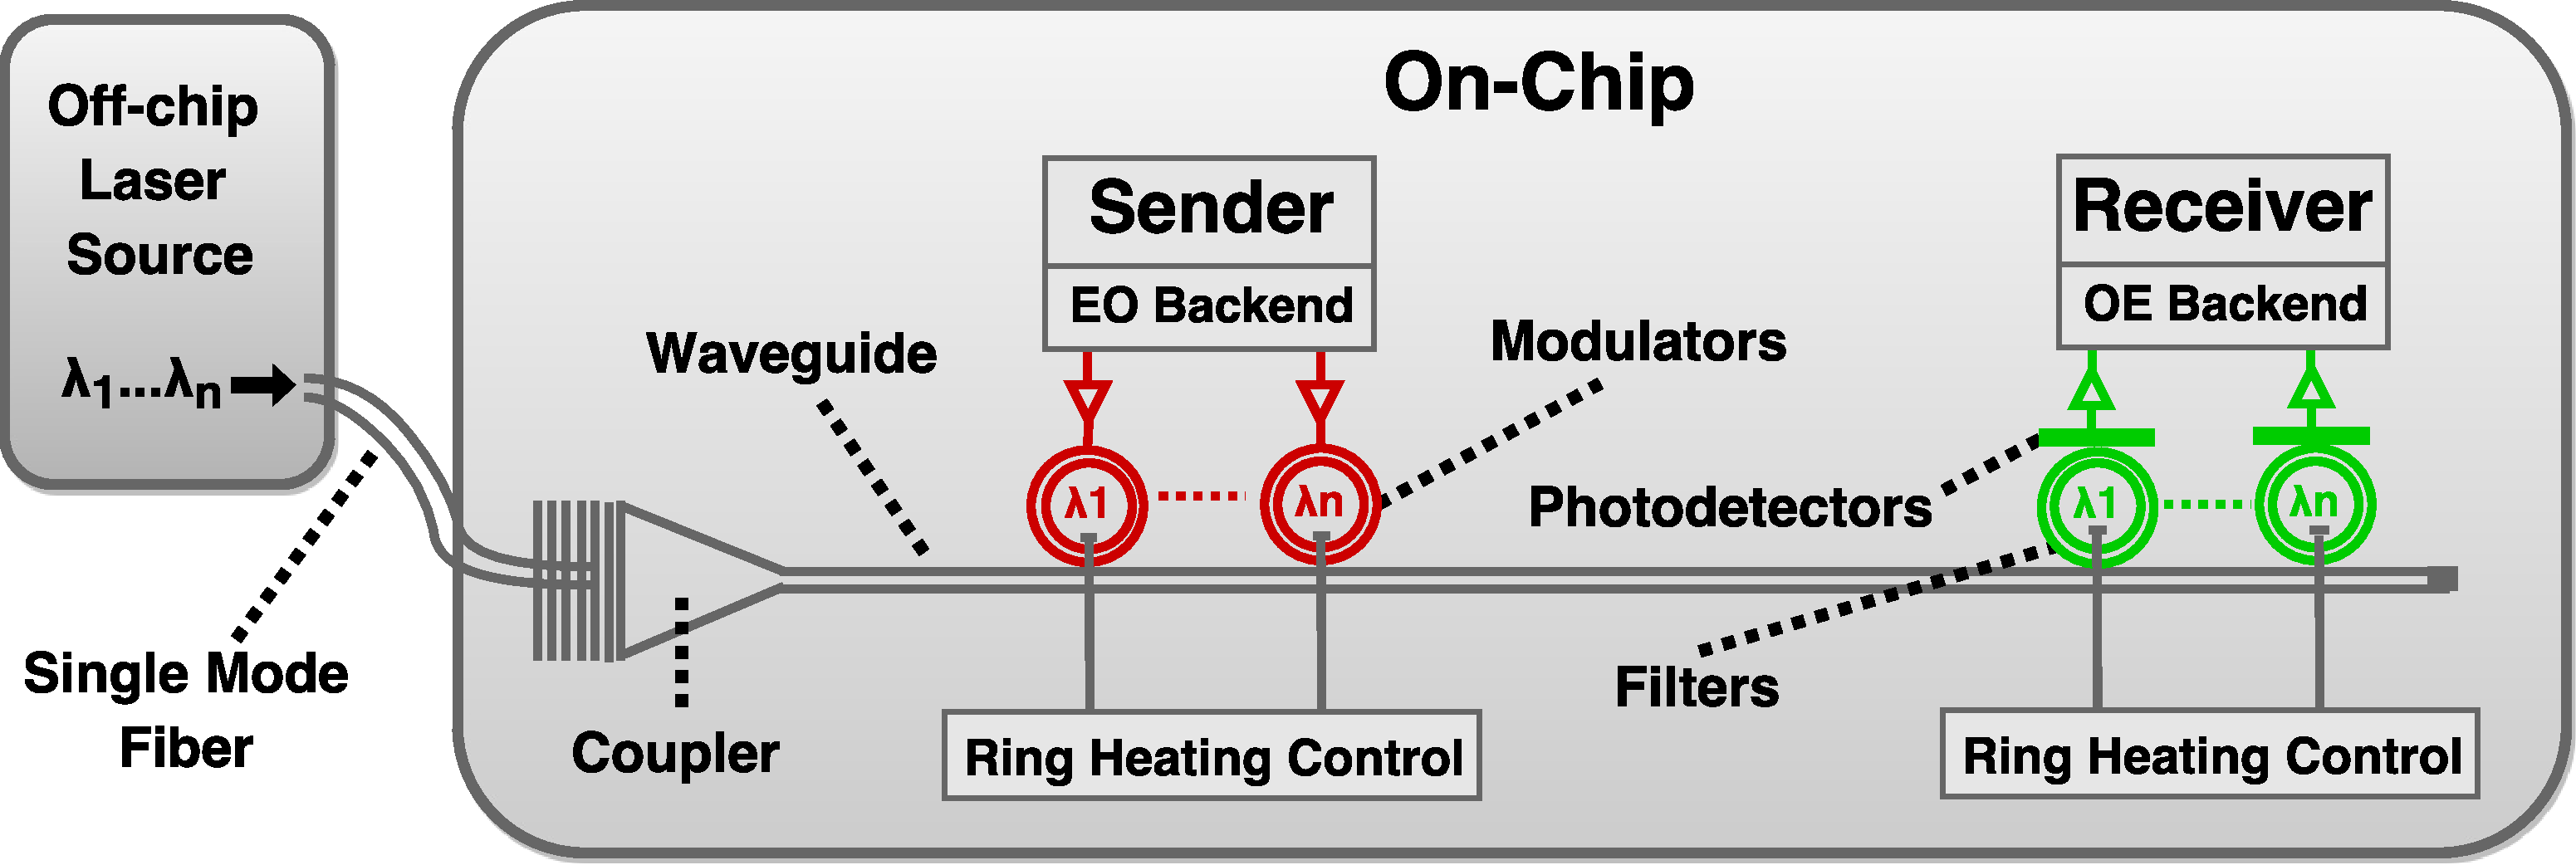
\includegraphics[width=\linewidth,clip]{latex/Figures/olink.pdf}
	\vspace{0.01cm}
	\caption[A Reference SiP Link]{A Reference SiP Link}
	\label{fig:olink} 
\end{figure}
Light generated from an off-chip laser is confined inside an optical fiber, which is then coupled into an on-chip waveguide. Modulators encode bits onto the optical medium (electrical-to-optical (EO) conversion), and filter-photodetector pairs extract the optical signal, performing optical-to-electrical (OE) conversion. Aside from steering particular wavelengths to a photodetector, MR filters are also deployed as switching devices since they allow to `drop' wavelengths from one waveguide to another, thereby allowing to implement wavelength-selective routing by strategically placing them between waveguides. \\
Optical signals can consist of multiple wavelengths ($\lambda _0 .. \lambda_n$) on which data can be transmitted in parallel--a technique commonly referred to as wavelength-division multiplexing (WDM). In order to exploit WDM, one modulator and MR filter per wavelength is needed at the sender and receiver, respectively. \\
MRs form the basis for both modulators and filters and are designed to respond to one particular wavelength channel (referred to as `resonance wavelength'); however, MRs are cyclic with the period--called the \textit{Free Spectral Range} (FSR)--meaning that an MR that drops wavelength $\lambda_i$ can also drop $\lambda_{i+ FSR*k}$ (with \textit{k} being an integer). A MR's resonance wavelength depends on device geometry/dimensions and the ambient temperature and variation thereof can cause the resonance wavelength to shift, effectively causing malfunctioning. While device mismatches during fabrication can be mitigated by MR trimming, protecting MRs from on-chip temperature variations requires integrated heaters ensuring thermo-optical control of each individual MR during operation. \\
Aside from ensuring correct behavior, integrated heaters can also be used deliberately to dynamically turn on/off MR filters. Changing the ambient temperature of a MR with heaters so that its resonance wavelength shifts beyond the free spectral range of all wavelengths on a link effectively allows to dynamically turn off (and on) a MR. Several previous studies leverage this approach to implement path setup and tear down functionality of circuit-switched optical networks based on wavelength-selective routing~\cite{bergman2014photonic}, which is also part of our proposed switching fabric. 

\subsection{Arrayed Waveguide Grating Router}\label{sec:awgr}
While all the wavelength routing functionality in an optical network could be implemented with MRs (as discussed above), networks solely relying on MRs to perform routing have several shortcomings, such as large power overheads for thermo-optical control of each MR, poor scalability (networks often require 1000s of MRs), excessive crosstalk, and the challenging task of finding a physical layout with low path losses~\cite{ramini2013contrasting}~\cite{boos2013proton}~\cite{hamedani2014qut}.\\
AWGRs overcome these challenges by providing scalable and low-loss wavelength routing on a passive platform that uses phase changes and constructive interference to enable an all-to-all $N \times N$ interconnection utilizing \textit{N} wavelengths and \textit{N} input and output waveguides~\cite{grani2017design}. Unlike MRs, AWGRs are less susceptible to temperature variations and do generally not require on-chip heating. 
In addition, recent advancements in CMOS-compatible SiN-based AWGRs enabled significantly reduced footprint ($<$1$mm^2$), low crosstalk ($<$-38dB) and loss ($<$2dB) values, giving AWGRs them a considerable edge to MR-based switching fabrics~\cite{shang2017low}. The physical layout of a fabricated SiN AWGR is illustrated in Figure~\ref{fig:awgrlayout}. \\
Figure \ref{fig:awgrmatrix} illustrates the wavelength distribution from the input to the output ports inside an $8\times 8$ AWGR. The wavelengths from each input port are evenly distributed to all output ports. 
\begin{figure*}[t!]
    \centering
        \begin{subfigure}[t]{0.18\linewidth}
        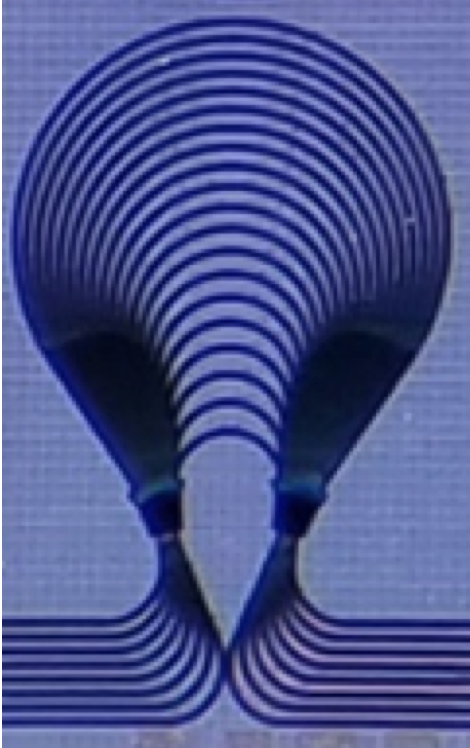
\includegraphics[width=\textwidth, clip]{Figures/awgrlayout.png}
        \caption{Physical Layout}
        		\label{fig:awgrlayout}
       \end{subfigure}
        \hspace{0.4cm}
        \begin{subfigure}[t]{0.46\linewidth}
        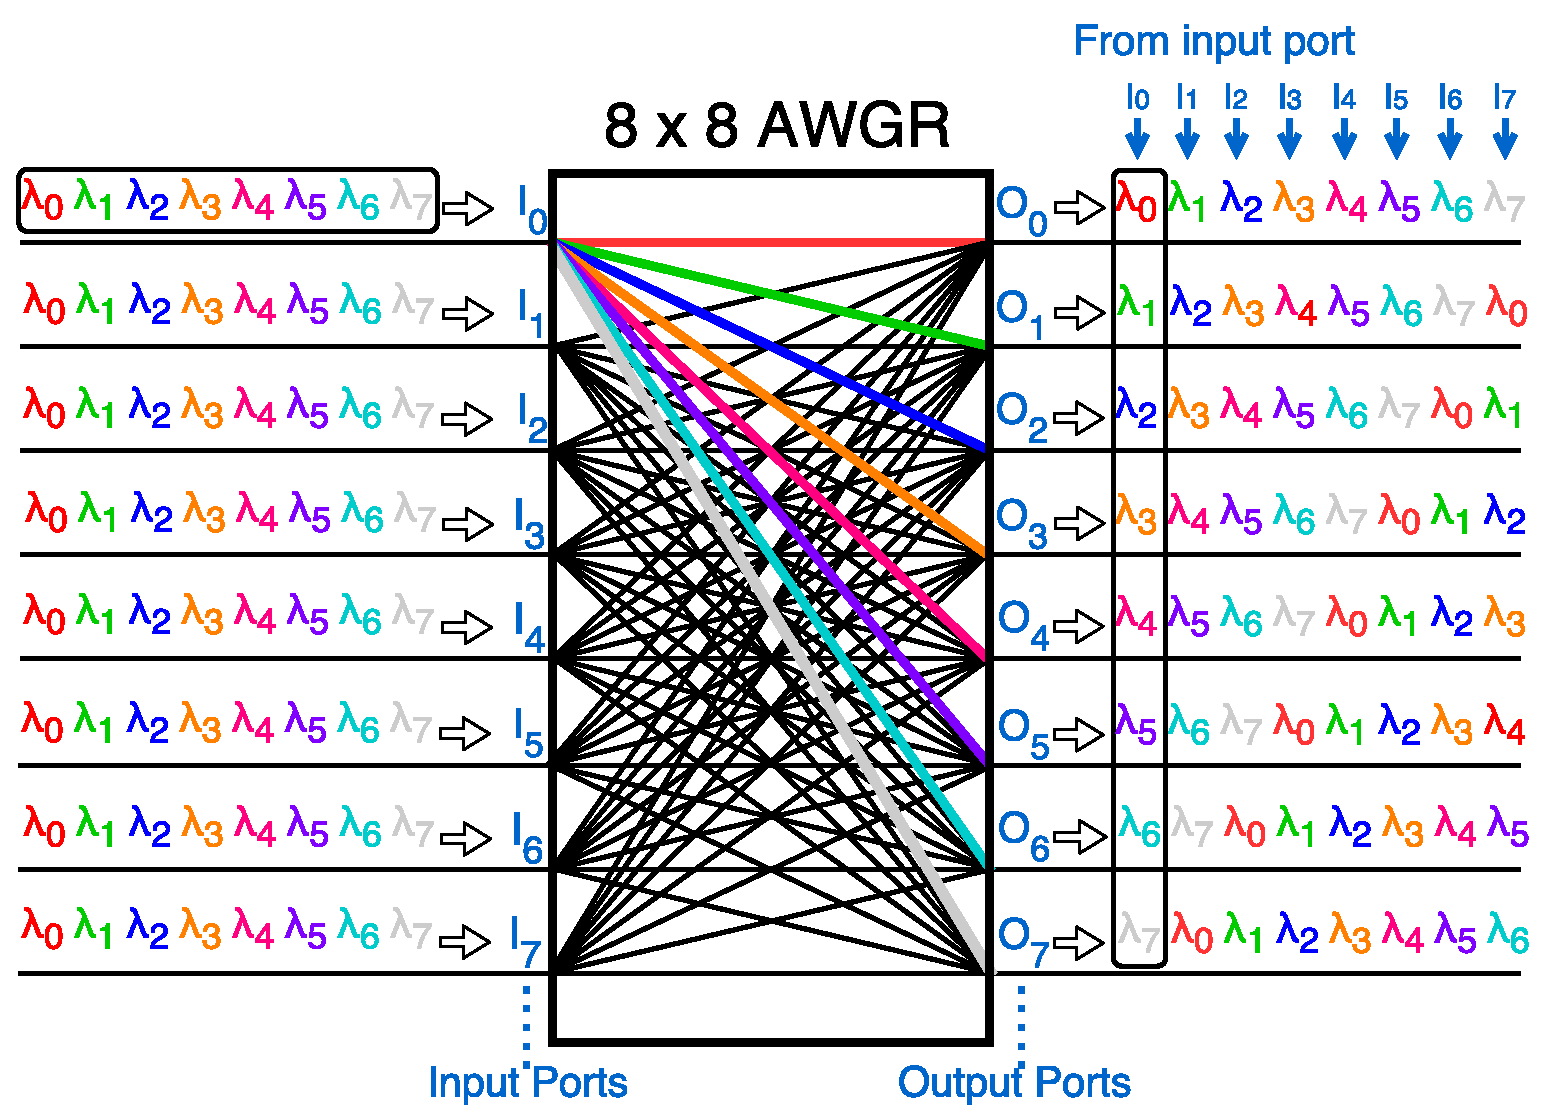
\includegraphics[width=\textwidth, clip]{Figures/awgr.pdf}
        \caption{Wavelength distribution inside an AWGR}
        		\label{fig:awgrmatrix}
    \end{subfigure}
        \hspace{0.4cm}
    \begin{subfigure}[t]{0.28\linewidth}
        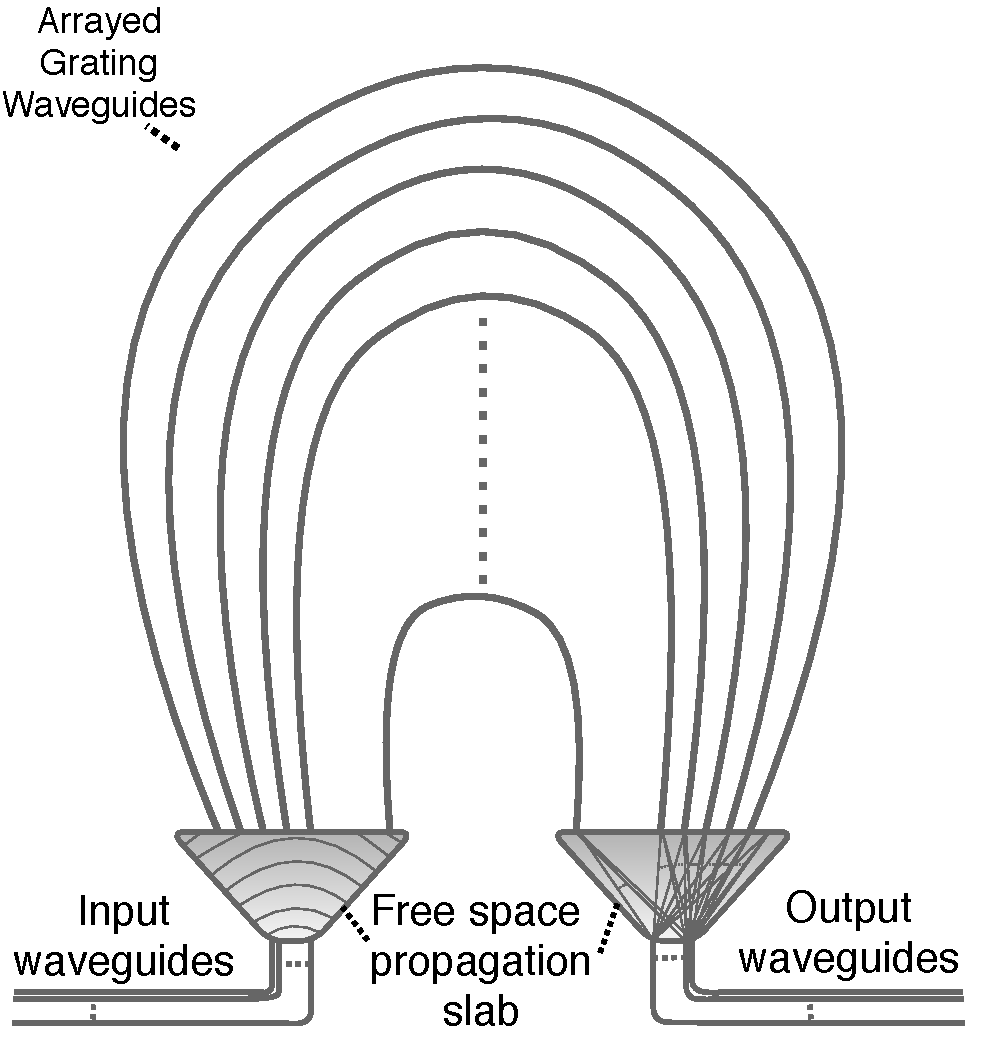
\includegraphics[width=\textwidth, clip]{Figures/awgrschematic.pdf}
        \caption{Schematic}
        		\label{fig:awgrcartoon}
    \end{subfigure}
    \caption[AWGR Structure and Switching Functionality]{Switching Functionality, Structure, and Layout of an 8$\times$8 AWGR}
\end{figure*}
This wavelength routing functionality is enabled by the constant phase change that each signal experiences when traversing the grating waveguides of an AWGR (see Figure~\ref{fig:awgrcartoon}) and is caused by the constant length increment of the grating waveguides. After traversing the grating waveguides, the wavelengths interfere constructively in the free space propagation region and get refocused at the output ports depending on their experienced phase shift.\\
It is important to note that, just like MRs, AWGRs are also cyclic with the period. Therefore, if input port \textit{i} can reach input port \textit{j} with wavelength $\lambda_{ij}$, \textit{i} can also reach \textit{j} with $\lambda_{ij + FSR*k}$ (with \textit{k} being an integer). This property has been exploited by previous studies to transmit multi-wavelength signals between source-destination pairs through an AWGR, referred to as \textit{bit-parallel AWGR}~\cite{grani2017bit}. 

\subsection{Color-blind switches}
*****TODO desribe and Compare MEMS/MZI/MRR crossbars *****\\
Problem: It's drawn in a figure 5 which doesn't appear until later ... TODO \\ 
\subsubsection{MEMS}
\subsubsection{MZI}
\subsubsection{MRR}
MEMS are color-blind SiP switches implementing a crossbar fabric with fast switching times, enabling rapid bandwidth reconfiguration. %Figure~\ref{fig:mems} (from~\cite{seok2016highly}) depicts an example $4 \times 4$ MEMS. 
%\begin{figure}[t!]
%        \includegraphics[width=\linewidth, clip]{Figures/mems.pdf}
%        \caption{From~\cite{seok2016highly}: (a) Depicts the structure of a MEMS switch with all its switching elements and input and output ports; (b) shows a close-up to a switching element, consisting of two layers of waveguides and a MEMS-Actuated Adiabatic Coupler; (c/d) illustrates the wavelength routing of the switching elements in OFF (c) and ON (d) state.}
  %      		\label{fig:mems}
%\end{figure}
Recently proposed MEMS switches proposed by researchers at UC Berkeley~\cite{seok2016highly} are particularly promising as they offer very low switching times (0.85$\mu$s), low on-chip insertion loss (8.5dB), low footprint ($1.9mm \times 1.9mm$ for a $16 \times 16$ MEMS), and, unlike MR-based fabrics, consume negligible on-chip power. \\
A MEMS has two layers of waveguides in crossbar mesh fabric and uses MEMS-actuated vertical adiabatic couplers as the switching elements (Figure~\ref{fig:mems}(b)). The optical operation bandwidth of adiabatic couplers ranges from 1400nm to 1700nm which is fully compatible with WDM networks. WDM signals entering an input port therefore either pass through to the `through ports' if all switching elements are in OFF state (Figure~ \ref{fig:mems}(c)) or are switched to one `drop port' if a switching element is in ON state.  \\
This structure allows each input port to reach every output port as long as the switching elements are (re)configured accordingly; however, MEMSs are color-blind switches and thus always switch \textit{all} wavelengths of a WDM to a certain output port. Variable bandwidth allocation is therefore not possible and each input can communicate only with one output at a time (simultaneous all-to-all connectivity like in AWGRs cannot be supported).  \\
In the following section, we show that MRs, AWGRs, and MEMS switches can, when co-integrated, be combined to form a powerful, highly-efficient, bandwidth-adaptive all-to-all interconnection fabric by exploiting the benefits of each device. 




\section{FlexLION}
\subsection{Target Interconnect Fabric}
The goal of our proposal FlexLION is to enable an all-to-all interconnection fabric in which each sender can dynamically allocate bandwidth to each of its output links based on an application's communication demand.\\
In an all-to-all network without configuration capability (as shown Figure~\ref{fig:logtopawgr}), each input port communicates with each output port with the same link bandwidth (for instance, a standard AWGR as in Figure~\ref{fig:awgrmatrix} provides such a fabric).
\begin{figure*}[t!]
    \centering
        \begin{subfigure}[t]{0.31\linewidth}
        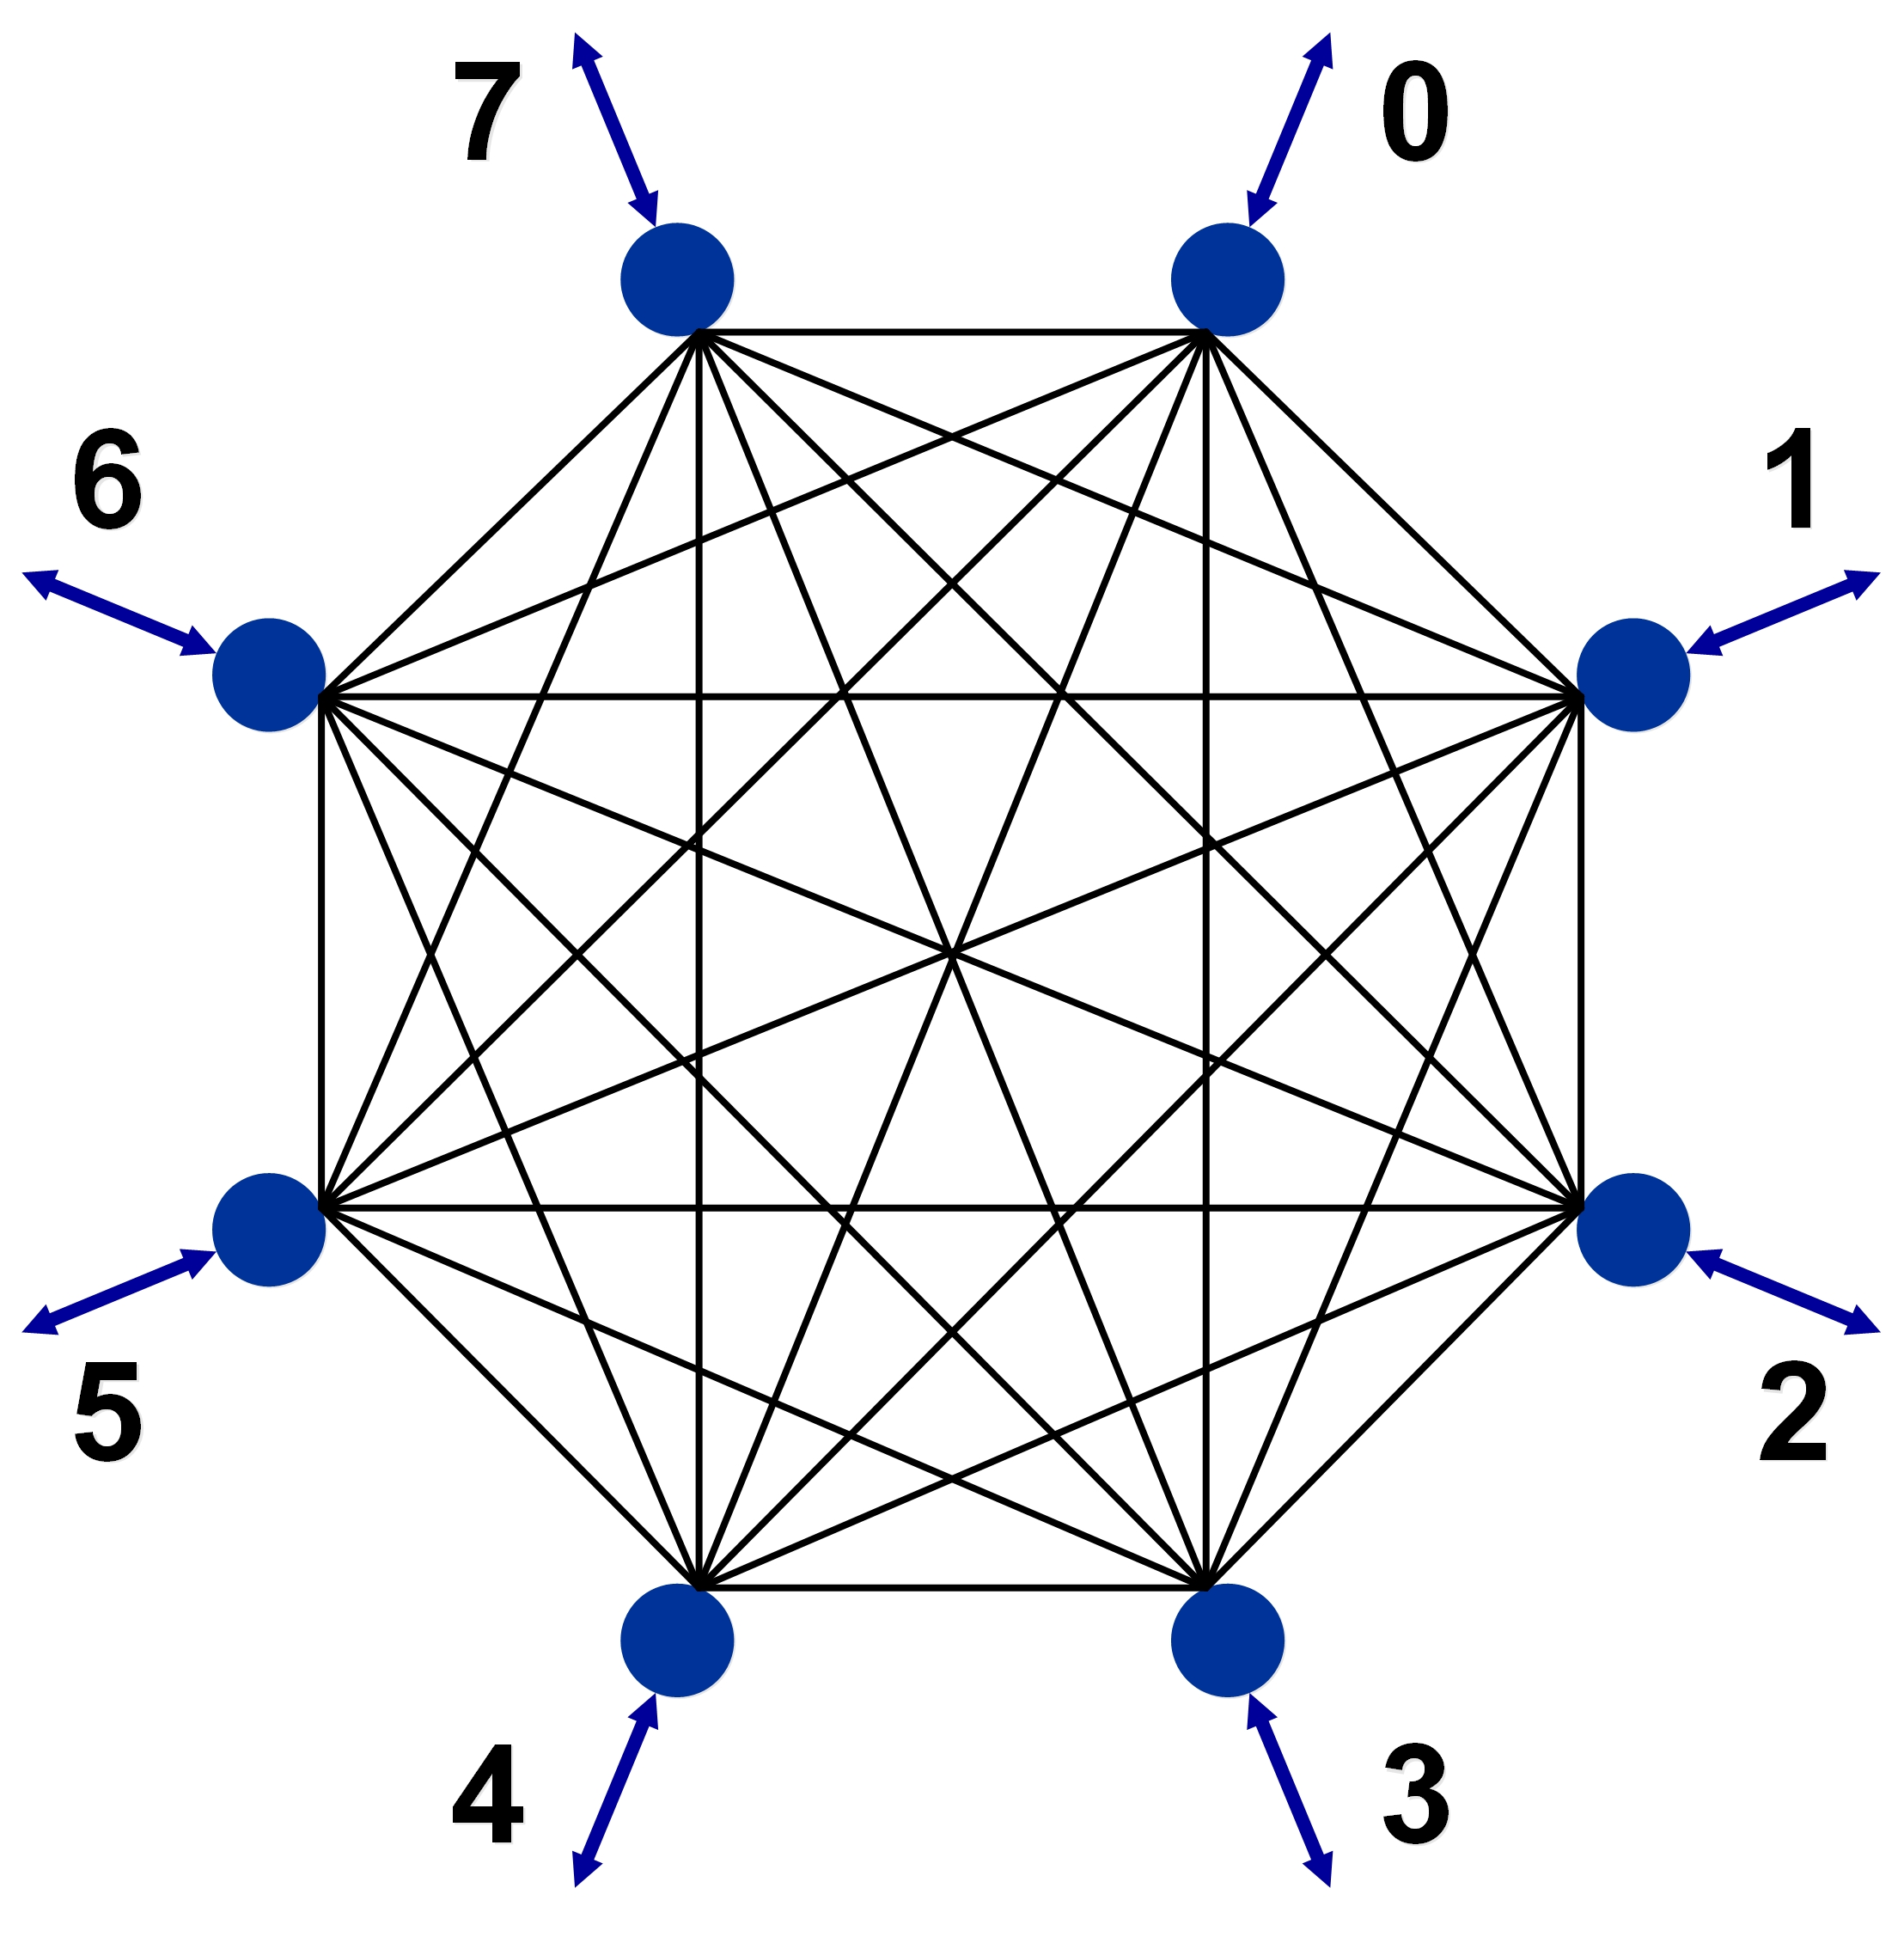
\includegraphics[width=\textwidth, clip]{Figures/logtopawgr.jpg}
        \caption{All-to-all network with uniform link bandwidth and no reconfiguration}
        		\label{fig:logtopawgr}
       \end{subfigure}
        \hspace{0.1cm}
        \begin{subfigure}[t]{0.31\linewidth}
        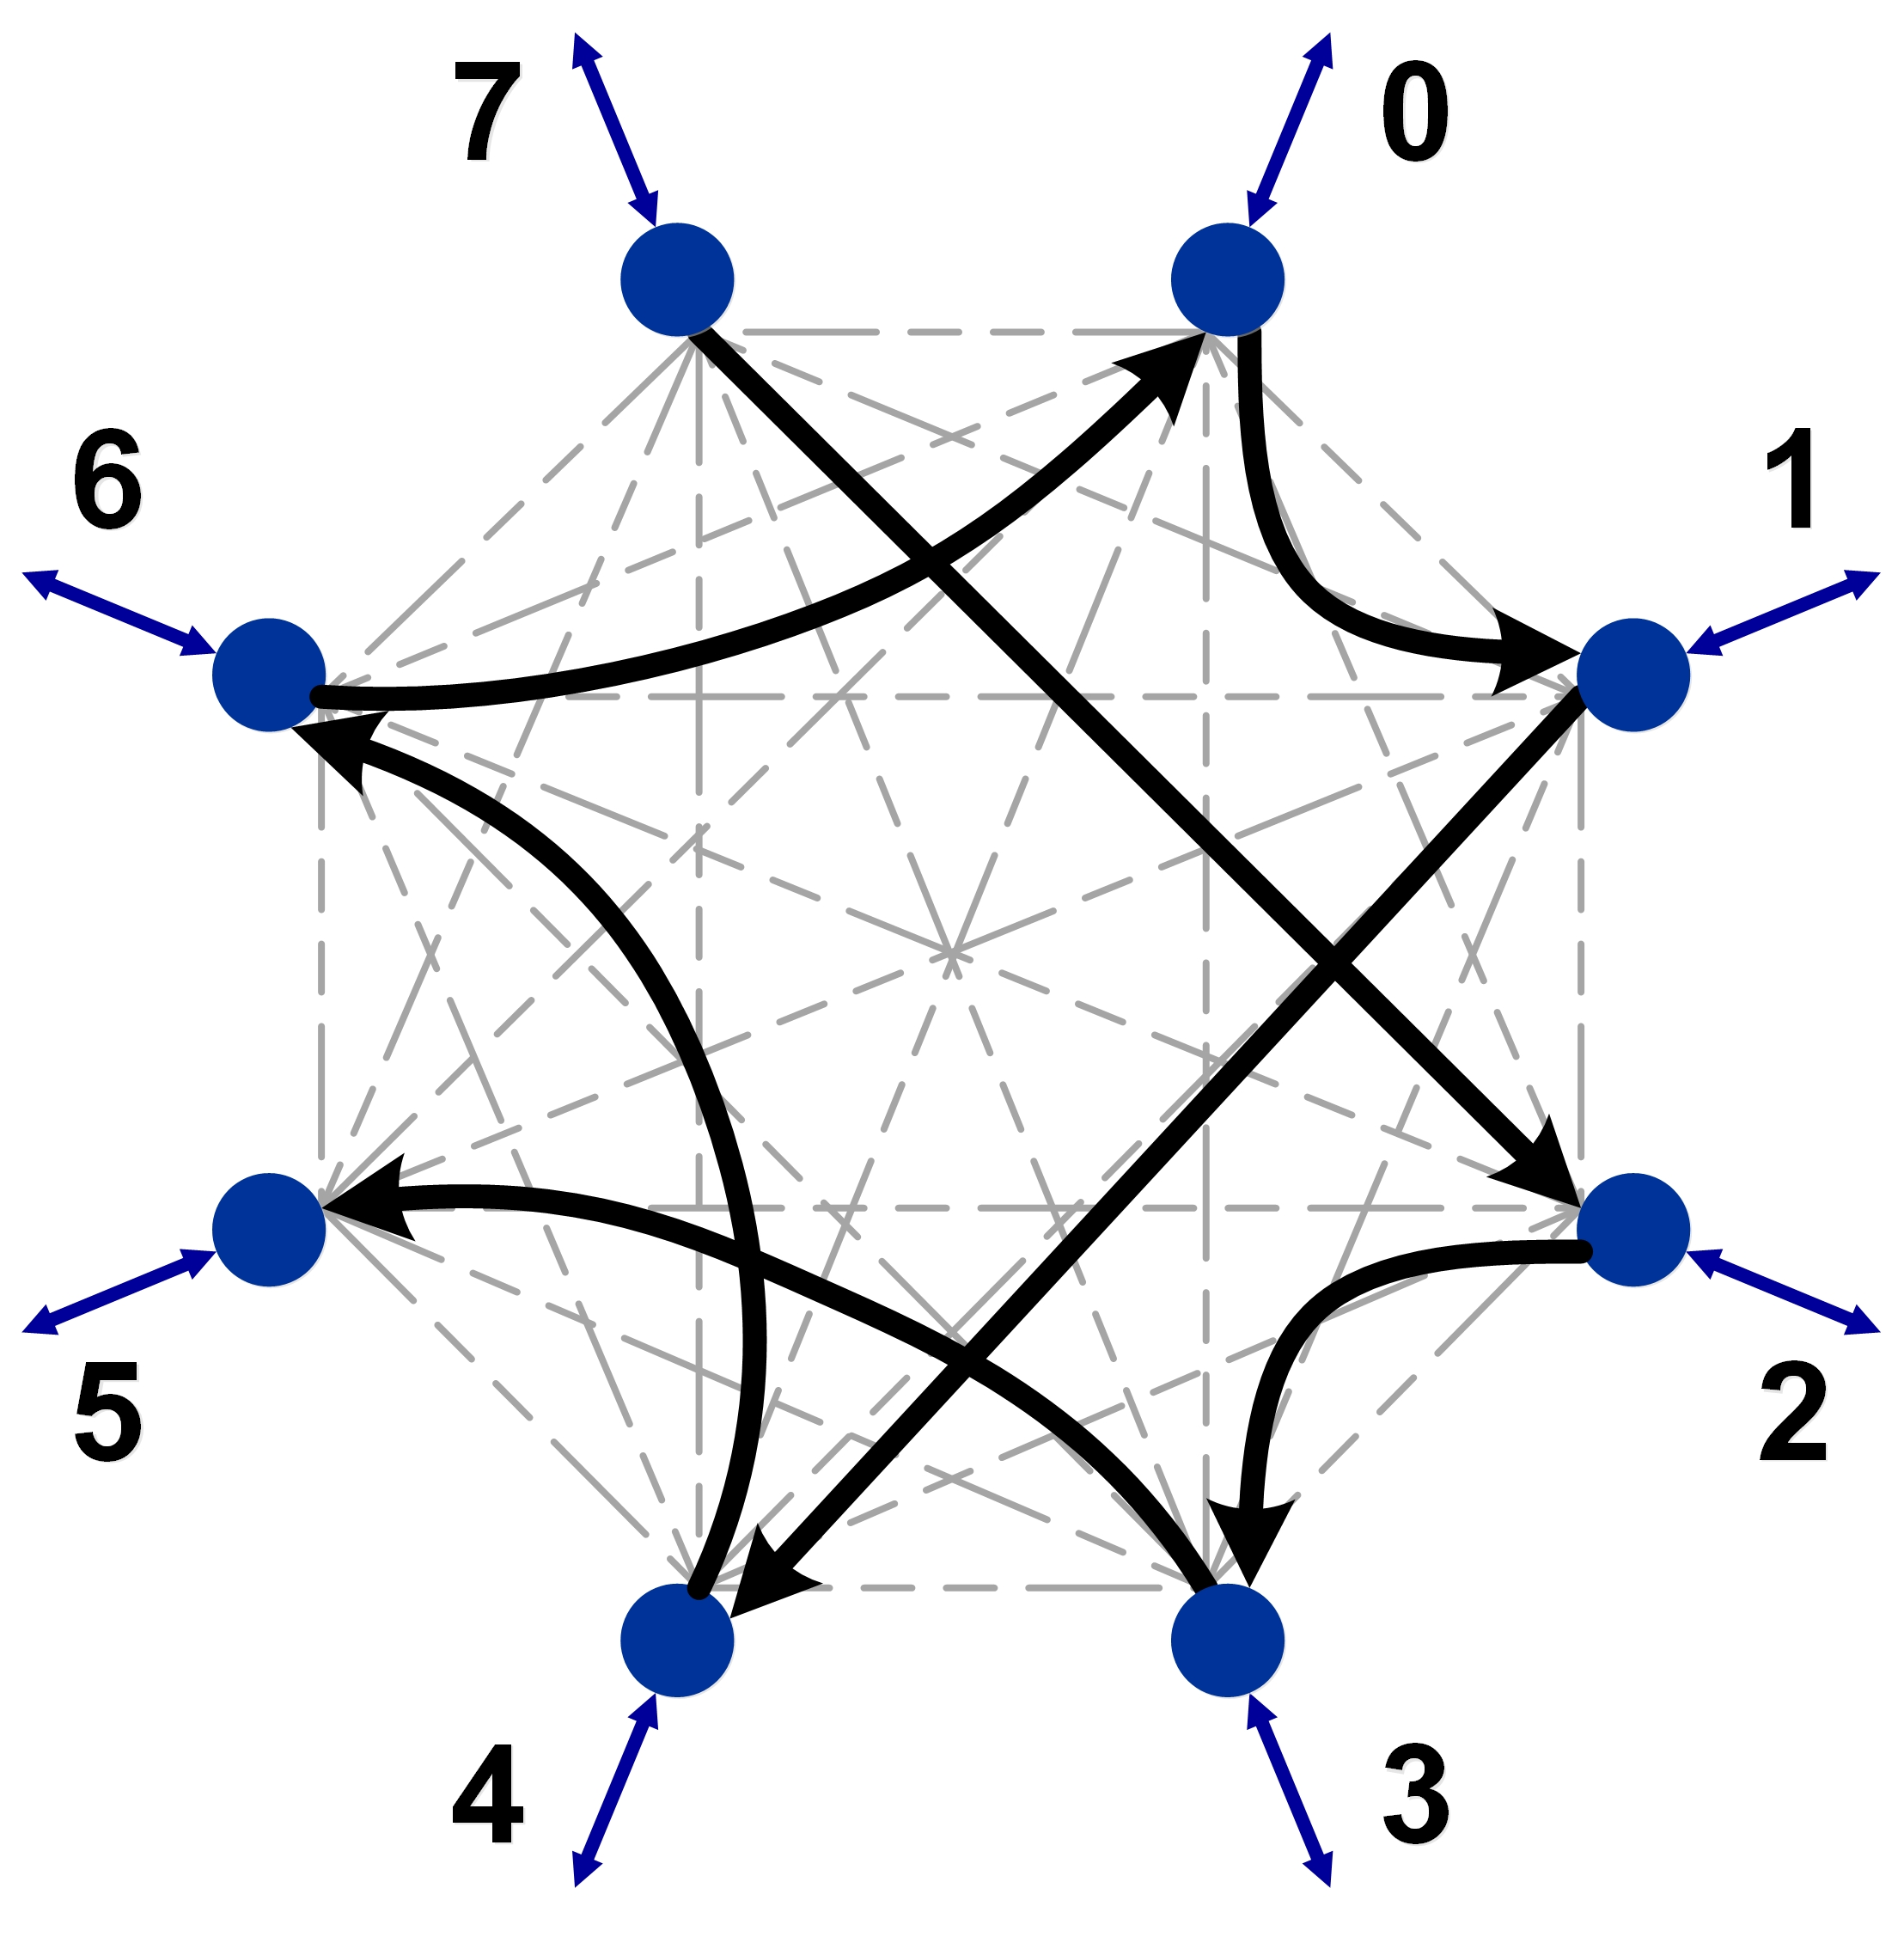
\includegraphics[width=\textwidth, clip]{Figures/logtopmems.jpg}
        \caption{Circuit-switched crossbar. Each sender can only send to one receiver using the entire available bandwidth; all other links are disconnected.}
        		\label{fig:logtopmems}
    \end{subfigure}
        \hspace{0.1cm}
    \begin{subfigure}[t]{0.31\linewidth}
        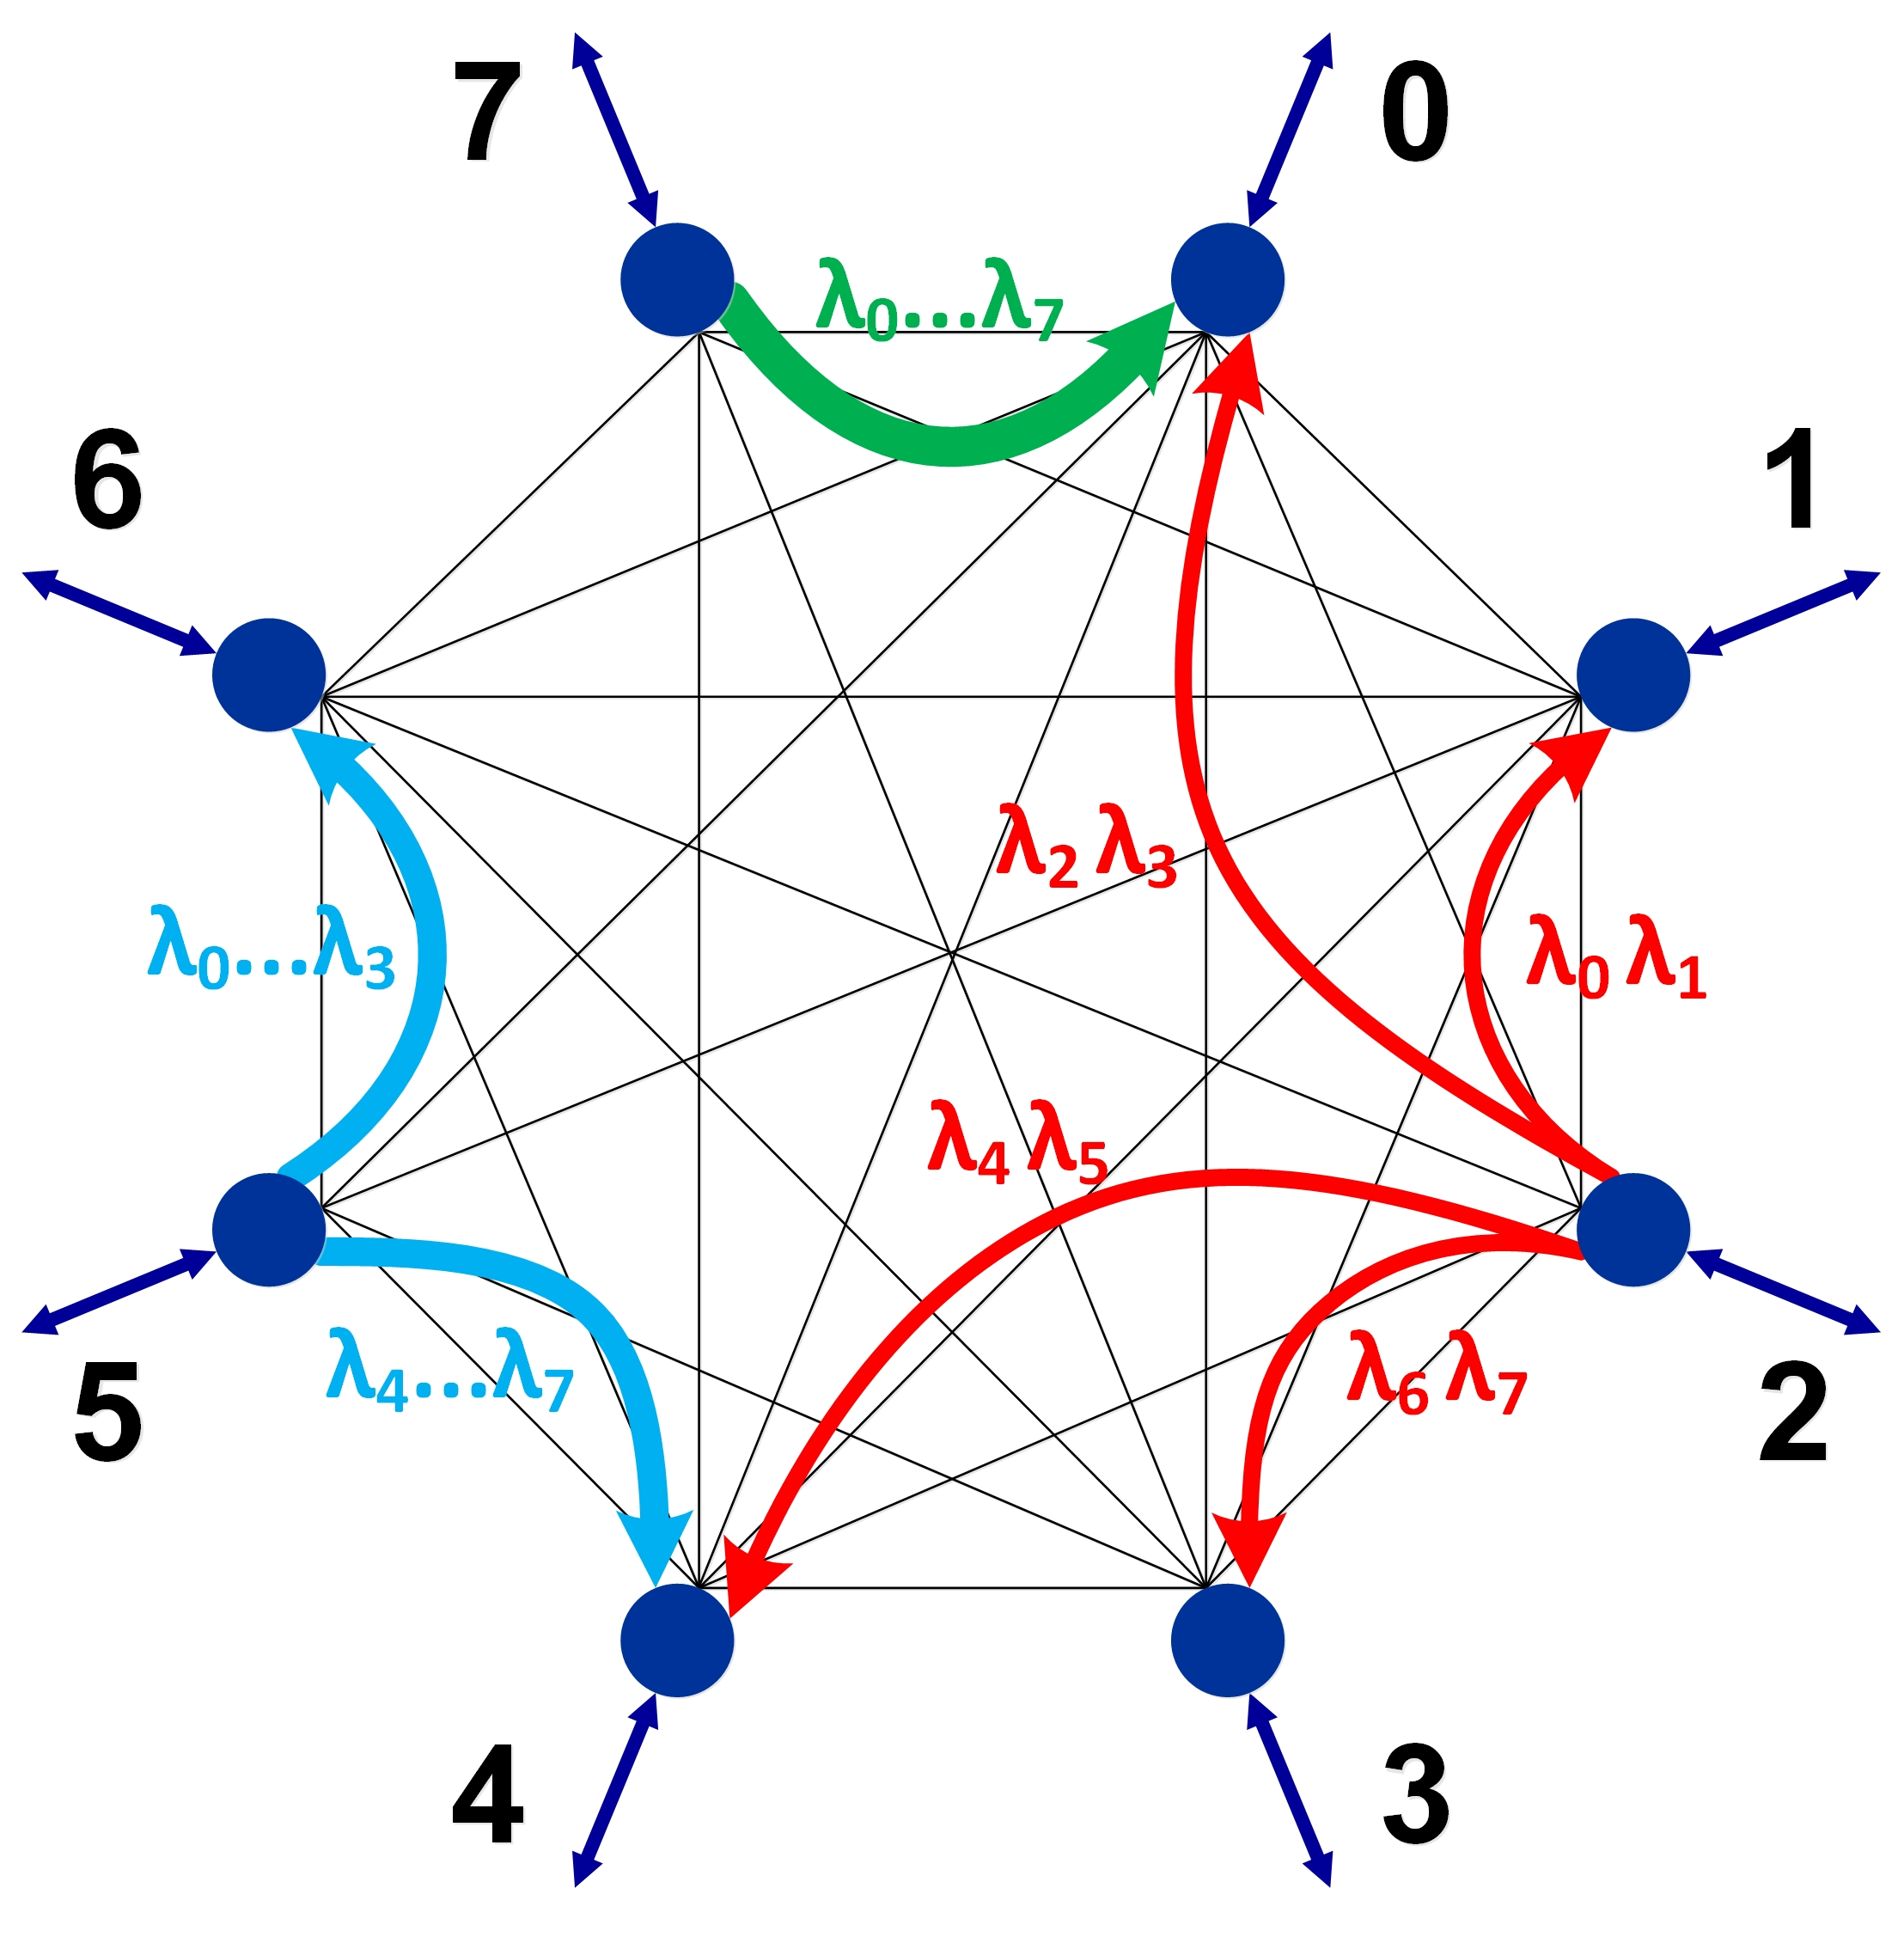
\includegraphics[width=\textwidth, clip]{Figures/logtopflex.jpg}
        \caption{All-to-all network with flexible bandwidth reconfiguration. Each available wavelength can be allocated to any link based on traffic demands.}
        		\label{fig:logtopflex}
    \end{subfigure}
    \caption[]{Logical all-to-all network topologies with different bandwidth reconfiguration capabilities}
\end{figure*}
Although all-to-all networks have the advantage of being a diameter-1 topology (and, in turn, offer minimal zero load latency), the bandwidth utilization in such networks is typically poor, leading to much of the network bandwidth and power being wasted on barely-utilized links. \\

This limitation can be overcome by exploiting WDM and wavelength-selective routing in SiPh components (instead of using independent all-to-all physical links between each sender-receiver pair). By leveraging this approach, each sender can have a pool of wavelengths available for data communication provided from a multi-wavelength laser and can allocate wavelengths to destinations based on the communication demands during an application. This allocation can be done by reconfiguring the optical network fabric, i.e.\ configuring which wavelengths are routed to which destinations, prior to executing a workload.\\
Previous proposals exploited wavelength routing by either using MEMS~\cite{seok2016highly} or broadband ring resonators~\cite{bergman2014photonic} to reconfigure the network; however, both approaches are based on broadband, color-blind SiP switching elements and can only route \textit{all} wavelengths from one node to another--effectively executing a circuit-switching mechanism allowing only point-to-point communication while all remaining connections are disconnected. This is illustrated in Figure~\ref{fig:logtopmems}. \\
Although these previous approaches might be useful in some scenarios (e.g., assigning all of the bandwidth to one destination to support large `elephant' flows in data centers~\cite{Farrington2010Helios}), in the vast majority of cases, traffic is more distributed and irregular in nature where one would still like to maintain connectivity to other nodes. In fact, superior performance metrics can be achieved if bandwidth reconfiguration would be more flexible and could support finer granularity between any sender-receiver pair. For instance, if a node A has to send 90\% of its traffic to node B and 10\% to node C (while other nodes are not communicated with) and have a pool of 10 wavelengths available, it would ideally allocate 9 wavelengths to node B and 1 to node C to achieve the highest performance. This could be enabled by reconfiguring the interconnection fabric to route 9 wavelengths from node A to node B and one wavelength to node C. This approach reduces the number of utilized fibers, can keep all nodes communicating with each other connected at all times, provides a higher degree of freedom for reconfiguring bandwidth compared to DVFS and could even be used in combination with DVFS for further variability. An example of a reconfigured network is shown in Figure~\ref{fig:logtopflex} in which multiple links have different numbers of wavelengths (and thus bandwidth) available for communication. FlexLION provides such a switching fabric, which will be introduced in the following. 

\subsection{FlexLION: Structure and Components}
*****TODO adjust *****\\
Therefore, we assume that ASIC switches are connected to FlexLIONS and use it as the communication fabric. In our design proposal, each switch ASIC is integrated on the same package as SiP transceivers, both placed and interconnected through an active SiP interposer, yielding tight integration and high energy efficiency (e.g., Intel's state-of-the-art 100G SiP transceivers require 35pJ/bit~\cite{intelsip}, while the recently demonstrated, tightly-integrated transceivers used in our study merely consume 0.55pJ/bit at 14nm~\cite{li201525}). Optical fibers connected to the SiP transceivers from each ASIC switch are coupled in and out of the die containing the FlexLIONS fabric, enabling all-to-all communication between all connected switches. The design in Figure~\ref{fig:flexdesign} envisions to place both the switch ASICs and FlexLIONS on the same board; however, since communication is optical and thus virtually distance-independent (in terms of latency and energy), system designers have a lot of freedom in placing the switches and are not restricted to mounting them on the same board.  \\
The FlexLIONS die contains the switching fabric that enables full connectivity between each input and output port and allows for maximum flexibility in bandwidth assignment. The AWGR provides all-to-all connectivity while the MRs and MEMS switching elements are utilized for the bandwidth reconfiguration. The most efficient and suitable approach for integrating all components within the same package is to use an active optical interposer. FlexLIONS easily fits on a 156$mm^2$ ($12mm \times 13mm$) interposer, a size that is readily available (for instance from AIM Photonics~\cite{aim}. In the following, we will describe the bandwidth reconfiguration mechanism in FlexLIONS. 

\subsection{Reconfiguration Mechanism}
Figure~\ref{fig:reconfexample} shows an example configuration of a 4-node FlexLION. 
\begin{figure*}[t!]
        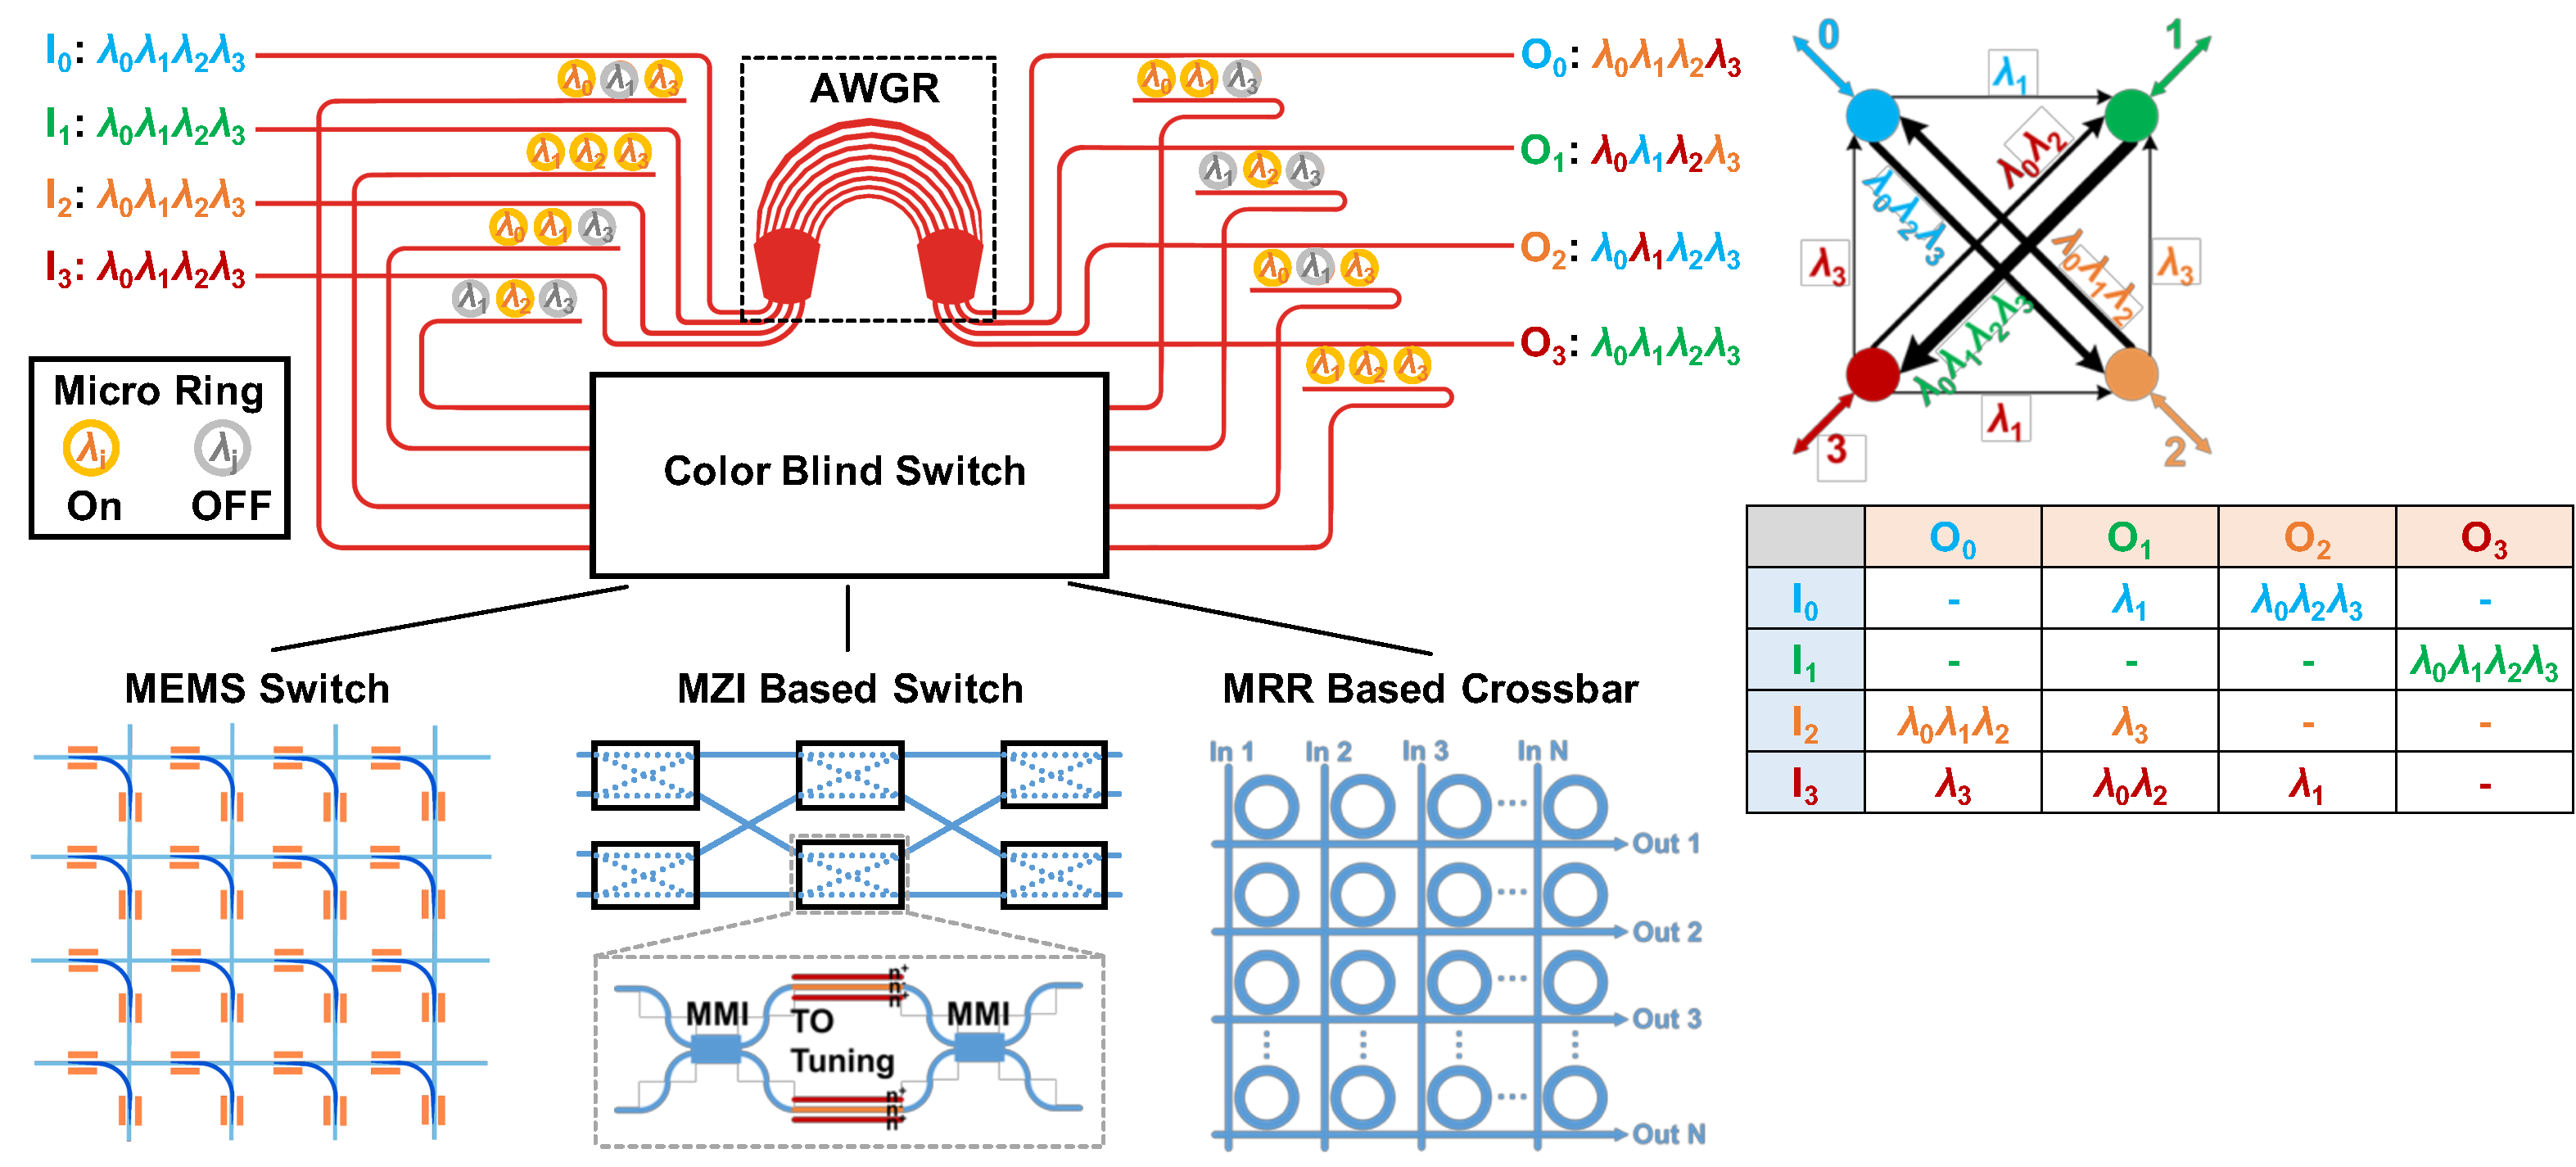
\includegraphics[width=\textwidth, clip]{Figures/reconf_example.pdf}
        \caption{Example of FlexLION reconfiguration functionality based on a $4\times4$ network.}
        		\label{fig:reconfexample}
\end{figure*}
The bandwidth reconfiguration is illustrated both in the logical topology in the top right corner and in the connectivity matrix in the bottom right corner. In all cases, the MRRs at the input and output waveguides, as well as the switching elements in the color-blind switch must be either turned ON or OFF, depending on what wavelength a sender wants to send to the destination node. Essentially, there are three different configuration cases: \\
1) A sender wants to evenly distribute its traffic (and thus the wavelengths/bandwidth) to all destination receivers. In this case, all MRRs at the input waveguide are turned OFF so that all wavelengths of the incoming WDM signal route through the AWGR, which evenly distributes the wavelengths to each output port (as described in Section~\ref{sec:awgr}). \\
2) A sender only wants to send all its traffic to the same destination: in this case, all MRRs at the input waveguide must be turned ON as they will then drop the wavelengths to the spatial switch. The adiabatic couplers in the MEMS responsible for steering wavelengths to the output port corresponding to the receiver must be turned ON (remember that the switching elements inside the MEMS are color-blind and thus always drop all wavelengths). Subsequently, the MRs at the output waveguides must be turned ON to drop the wavelength to the desired output port. This is illustrated in Figure~\ref{fig:reconfexample} from input $I_1$ to output $O_1$.  \\
3) A sender has different traffic demands for different destination nodes (see Figure~\ref{fig:reconfexample} $I_0->O_1$/$O_2$, $I_2->O_0$/$O_1$, $I_3->O_0$/$O_1$/$O_2$). In that case, there are two possibilities: either the AWGR routes a wavelength to the desired output port, in which case the MRR at the input waveguide must be turned OFF to allow the signal to go through the AWGR. Otherwise, the MRRs at the input waveguides corresponding to the wavelengths destined to the output waveguide must be turned ON in combination with the correct switching elements of the color-blind switch and the MRRs at the output waveguides. \\
Note that a reconfigurable fabric like FlexLION has one input link/fiber and one output link/fiber to each node in the network. Given that each node has only one input port, the wavelength assignment/reconfiguration must occur so that two or more senders cannot send to the same destination node on the same wavelengths (to avoid destructive interference when two signals on the same wavelength arrive at a receiver simultaneously). Therefore, such a switching fabric, though providing all-to-all connectivity, does not represent a strict point-to-point, contention-less topology, and a reconfiguration mechanism must take into account all senders, receivers, and bandwidth demands to assign wavelengths to senders while preventing destructive interference. 
\subsection{Reconfiguration from a System Perspective}
This paper proposes a novel interconnection fabric providing reconfiguration capability with compact footprint at low loss and heating requirements; however, we acknowledge that from a system perspective, performing reconfiguration is an important research area on its own and deserves detailed attention--especially as arbitrating HPC networks becomes increasingly complex as they scale up. \\
Several previous works have studied the challenge of efficiently reconfiguring an interconnection fabric in HPC system. Most notably, Bergman's research group has put much focus on developing a system with the required hardware and software to reconfigure the interconnection of a SiPh switch~\cite{shen2018software}~\cite{shen2017software}~\cite{shen2018autonomous}~\cite{shen2018accelerating}~\cite{bahadori2018design}. In particular, they successfully demonstrated a testbed system based on preconfigured FPGAs which are on the one side connected to the SiPh switch via a Digital-to-Analog converter (DAC) (which controls the MRRs via hard-coded voltage/current levels to tune the MRRs to respond to certain wavelengths) and on the other side to a central SDN controller that controls the routing tables of the electronic switches through the OpenFlow protocol~\cite{shen2018accelerating}. This traffic-driven approach oversees a switches input queues and reconfigures of the SiPh switch in a synchronised fashion to control the flow of packets while reconfiguring the physical topology. \\
This testbed performs reconfiguration of the entire control plane in 224$\mu$s and the communication between the SDN-FPGA controllers and SDN-electrical switch (223$\mu$s~\cite{shen2018software}), which occurs over a 1G Ethernet, represent the performance bottleneck. The actual reconfiguration/tuning of the SiPh components in the optical switch merely take 12$\mu$s (most of which due to the slow sub-MHz sampling speed of the DAC and the fact that the DAC is on a separate board)~\cite{shen2018software}. \\
While Bergman's work has high significance as it is the first to demonstrate a working system with a SiPh switch, much of the reconfiguration time could probably be significantly reduced by co-integrating the FPGA controller, DAC, and SiPh components in the same package (rather than on different boards), using faster sampling speeds for the DAC, using SiPh transceivers rather than 1G Ethernet for SDN-FPGA controller communication, or performing reconfiguration based a priori knowledge about a workloads communication patterns (rather than using OpenFlow). Regardless of the challenges, we point out that the reconfiguration of the SiPh components (be it MRRs, MZIs, or MEMS) are not on the critical path in terms of reconfiguration latency. 

\subsection{Utilization in HPC Center Network}
We study the impact FlexLION can have on inter-rack networks. The vast majority of high-performance data center networks are based on tree-based topologies, most prominently fat trees or clos topologies~\cite{kachris2012survey}, as they provide good scalability and load balancing properties. To save resources and power, or to adapt to current network utilization, oversubscription is a technique often used in tree-based networks in which the next tree stage only has a fraction of output links/bandwidth of the previous stage. \\
Figure~\ref{fig:networktopologies} illustrates example topologies supporting 256 nodes~\footnote{Note that the number of nodes supported by a HPC center network can vary based on the system scale. As a reference, Intel's Omni-path Director Class switches support either 192 or 768 port units~\cite{inteldir}.} comparing an HPC center network with FlexLIONS to legacy fat tree based topologies. 
\begin{figure*}[t!]
    \centering
        \begin{subfigure}[t]{0.28\linewidth}
        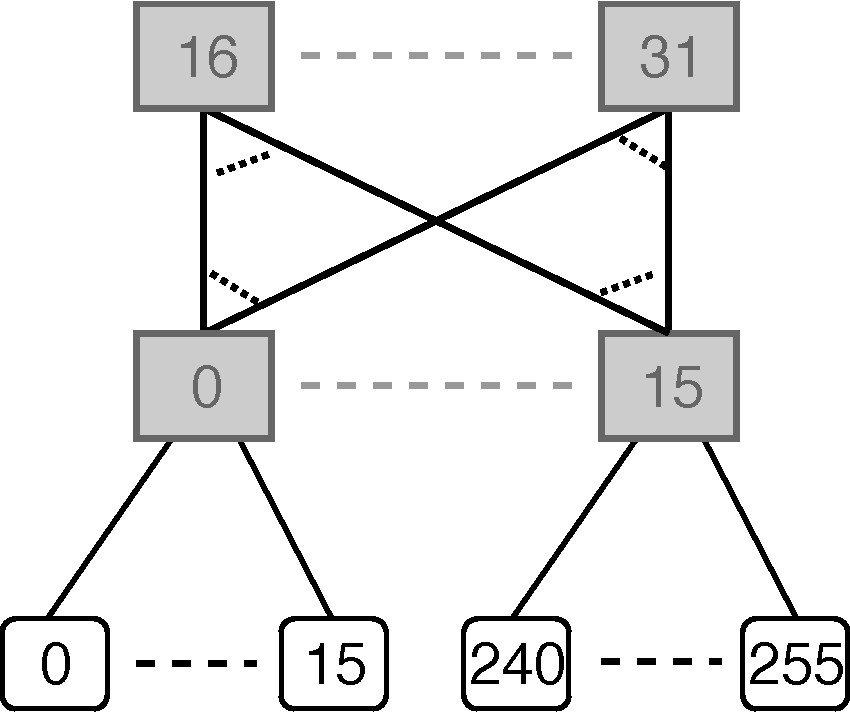
\includegraphics[width=\textwidth, clip]{Figures/treeFull.pdf}
        \caption{}
        		\label{fig:treeFull}
    \end{subfigure}
        \hspace{0.5cm}
    \begin{subfigure}[t]{0.28\linewidth}
        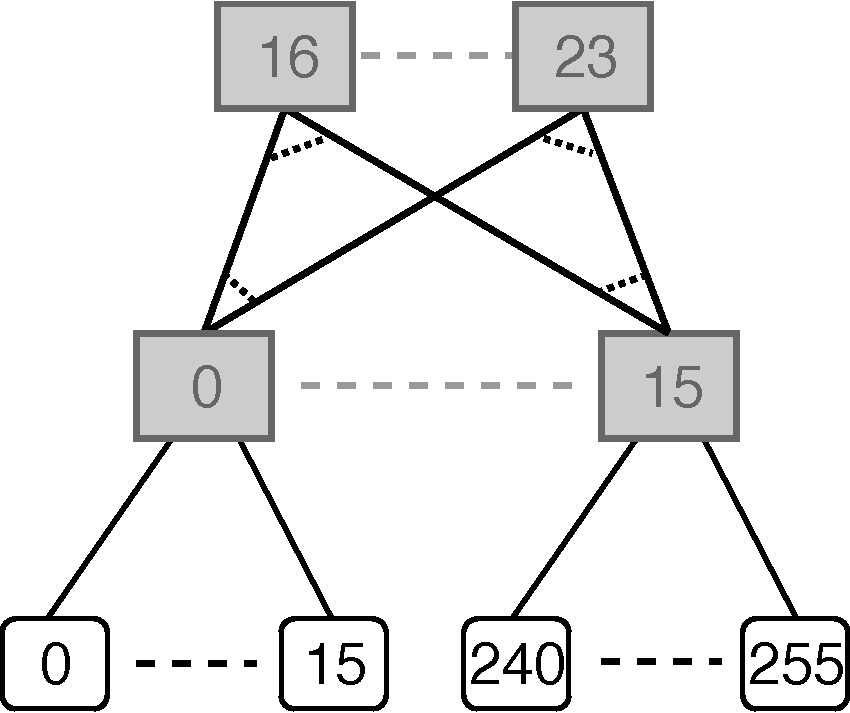
\includegraphics[width=\textwidth, clip]{Figures/treeHalf.pdf}
        \caption{}
        		\label{fig:treeHalf}
    \end{subfigure}
    \hspace{0.5cm}
    \begin{subfigure}[t]{0.28\linewidth}
        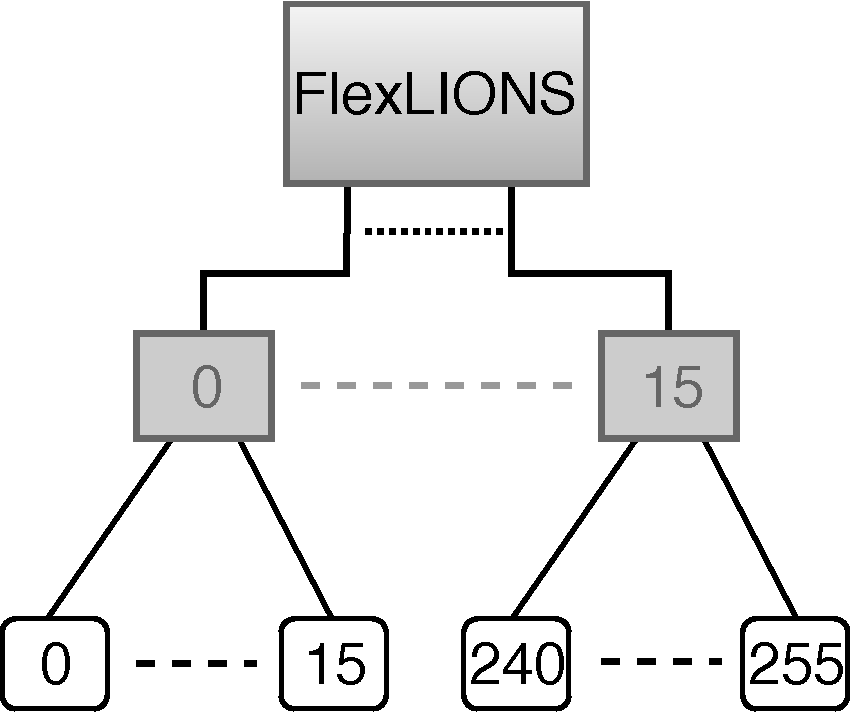
\includegraphics[width=\textwidth, clip]{Figures/flexlionIncenter.pdf}
        \caption{}
        		\label{fig:flexlionIncenter}
       \end{subfigure}
    \caption[]{HPC network topologies supporting 256 nodes: (a) Fat Tree, (b) Fat Tree with oversubscription of 2, (c) FlexLIONS}
    \label{fig:networktopologies}
\end{figure*}
Figure~\ref{fig:treeFull} depicts a 2-layer fat tree (`Fat Tree') without oversubscription, consisting of 32 32-port switches and 640 transceivers. Figure~\ref{fig:treeHalf} shows the same network, but with an oversubscription of two (`Fat Tree 2:1'), i.e.\ the number of switches on the second layer and thus the number of outgoing links on the first layer is half of that of a full Fat Tree. Figure~\ref{fig:flexlionIncenter} shows a 256-node HPC network with FlexLION, which requires 16 32-port switches, 512 transceivers, and the FlexLION fabric. 32-port switches are widely deployed and commercially available by vendors like Mellanox or Intel~\cite{mellanox}~\cite{intelomnipath}. Note that classic fat trees in HPC networks typically consist of three layers (edge, aggregate, and core switches); however, for our 256-node study we hypothesize that a 2-layer fat tree suffices to satisfy the bandwidth demands and provides more competitive zero load latency compared to the 1-layer FlexLION based network. A comparison of the properties of these three networks is listed in Table ~\ref{tab:properties}. \\
\begin{table}[]
\caption{Resource requirements of the HPC networks under investigation}
\label{tab:properties}
\centering
\begin{tabular}{@{}c|ccc@{}}
\toprule
                  & Fat Tree & Fat Tree 2:1 & FlexLIONS \\ \midrule
\#Switches     & 32       & 24           & 16        \\
\#Transceivers & 1024     & 640          & 512       \\
Link data rate & 100G     & 100G         & 100G      \\
Bisection BW   & 25.6Tb   & 12.8Tb       & 25.6Tb   \\ \bottomrule
\end{tabular}
\end{table}
One main benefit of FlexLION is that its reconfiguration capability can make efficient use of the available bandwidth and might thus provide satisfactory performs metrics without requiring a multi-stage network like trees for load balancing. In HPC center networks, the latency imposed by additional hops through a switches can have a significant impact on system performance. For instance, the most competitive design in terms of latency currently available is Intel's Omni-path ASIC switch which requires 100ns for switch traversal~\cite{intelomnipath}. With this value, the FlexLION network would reduce zero load latency from 300ns to 200ns compared to a two stage tree, which can be significant, especially in low utilization phases where the bandwidth is not stressed. Moreover, FlexLION reduces the total number of required switches and transceivers, while providing similar bisection bandwidth. In  Section 4, we will evaluate whether the bandwidth reconfiguration of FlexLION indeed allows similar performance as tree-based networks while significantly reducing resources, power, and zero load latency. 

\subsection{Design Considerations and Scalability}
The previous examples introducing FlexLION were based on four wavelengths per input port--one for each output port. The comparison in Table~\ref{tab:properties} is based on 100Gb/s per link since this is a common data rate for state-of-the-art HPC interconnects (e.g., Intel's SiP transceiver offers 100Gb/s data rate (4 wavelengths at 25Gb/s modulation rate)~\cite{intelsip}. Since data rates around 25Gb/s modulation rate offer the highest energy efficiency, FlexLION must be able to support multiple wavelengths (in this example, 4) for each receiver to support 100Gb/s communication on each link. In order to support bit-level parallelism of 4, we exploit the cyclic dependence of MRRs' resonant wavelengths and AWGRs and provide each sender with the wavelengths: $\lambda_{0}$, $\lambda_{0+FSR}$, $\lambda_{0+2*FSR}$, $\lambda_{0+3*FSR}$, ...$\lambda_{n}$, $\lambda_{n+FSR}$, $\lambda_{n+2*FSR}$, $\lambda_{n+3*FSR}$. For a 16-port FlexLIONS, each input port must be provided with $16 \times 4 = 64$ wavelengths. \\
The network in Figure~\ref{fig:flexlionIncenter} would require a 16-port FlexLION switching fabric and in turn a $16 \times 16$-port AWGR and spatial switch--both of which have been demonstrated and do not exhibit scalability problems for this port count~\cite{shang2017low}~\cite{seok2016large}. In fact, SiN AWGRs used in FlexLION can scale up to 64 ports before crosstalk penalties become a considerable issue. MEMS switches have also been demonstrated to scale up to 64 ports without issues (albeit with increased, but still acceptable, area footprint of $7mm \times 7mm$) ~\cite{seok2016large}.\\
In order to provide full reconfiguration capability, each input port requires one MRR for each wavelength but one (one wavelength will always be routed to a desired output port through the AWGR). That means, for 64 wavelengths per input/output port, this would make $63 \times 2 = 126$ MRRs per input/output, and $16 \times 126 = 2016$ MRRs. Alternatively, it is also possible to reduce the number of wavelengths that a sender can reconfigure and thereby reduce the number of MRRs needed. For instance, if a node can only reconfigure half the number of total wavelength, $16 \times 31 \times 2 = 992$ MRRs. If only a quarter the number of total wavelengths can be reconfigured, only 480 MRRs are needed. However, physically implementing 2016 MRRs (for fully reconfigurability of each wavelength) in a SiPh process should not pose any issues in terms of area or energy. The scalability of FlexLION and all its components discussed above is summarized in Table~\ref{fig:flexscale} for up 64 ports. 
\begin{table}[]
\centering
\caption{FlexLION resource requirements for scaling to higher port counts (assuming 4 wavelengths at 25Gb/s for a 100Gb/s link and full bandwidth reconfigurability)}
\label{fig:flexscale}
\begin{tabular}{@{}c|cccc@{}}
\toprule
              & \multicolumn{3}{c}{FlexLION \#Ports} &  \\ \midrule
 Component             & 16 ports         & 32 ports        & 64 ports       &  \\ \midrule
AWGR          & 16x16      & 32x32      & 64x64     &  \\
MEMS          & 16x16      & 32x32      & 64x64     &  \\
\#MRRs         & 2016       & 4032       & 8064      &  \\
\#Wavelengths & 64         & 128        & 256       &  \\ \bottomrule
\end{tabular}
\end{table}

\section{Evaluation}
\subsection{Methodology}
We experimentally evaluate FlexLION implementing the rack-level interconnect from the previous section and compare it to the discussed tree-based topologies. We stick to the same network configuration from Table~\ref{tab:properties} and Figure~\ref{fig:networktopologies} for all the networks and thus study the interconnect of a 256-node network. We use gem5~\cite{binkert2011gem5} with Garnet2.0~\cite{agarwal2009garnet} for detailed performance simulation. We evaluate the network under a range of traditional synthetic traffic patterns (uniform random, bit complement, tornado, shuffle) to stress all corner cases of the topologies. \\
To compare FlexLION with the most aggressive baseline, we model the power consumption and latency of the switches based on state-of-the-art commercially-available data center switches, which consume 95W power and offer a 100ns switch traversal latency~\cite{intelomnipath}~\cite{mellanox}. We consider two transceiver technologies in our study: 1) Intel's SiPh transceivers which consume 35pJ/bit with 100G line rate~\cite{intelsip} and represent the most advanced commercially-available technology, and 2) tightly-integrated electronic-photonic co-designed transceivers have been demonstrated at the research level that can consume as little as 2pJ/bit in a 65nm technology~\cite{li201525}\footnote{Technology-scaling with SPICE models show 0.55pJ/bit at 14nm.}. Table~\ref{fig:sipparameter} lists the parameters we used for power modeling of the SiPh components(transceivers and FlexLION). While we model our FlexLION only with SiPh transceivers 2), we model the legacy fat tree topologies with both transceiver types 1) and 2). These comparisons allow to reveal the power savings of FlexLION in comparison to legacy topologies with the same transceiver technology and to illustrate the total power saving potential that FlexLION provides compared to state-of-the-art topologies (i.e., fat trees) with the best commercially-available transceivers. 
\begin{table}[]
\centering
\caption{SiP Technology Parameters}
\label{fig:sipparameter}
\begin{tabular}{@{}lllll@{}}
\toprule
Parameter            & Value     & Parameter      & Value  &  \\ \midrule
Laser Efficiency     & 14\%      & Coupler Loss   & 1 dB   &  \\
Waveguide Loss       & 2.2 dB/cm & Photodiode     & 0.1 dB &  \\
Receiver Sensitivity & -17.7 dBm & Modulator Loss & 1 dB   &  \\
Add-drop Filter Loss & 1.5 dB    & Power Margin   & 3 dB   &  \\ \bottomrule
\end{tabular}
\end{table}
We study FlexLION with different degrees of reconfigurability to expose the benefits and drawbacks of providing different levels of flexibility (i.e., as discussed earlier, number of MRRs vs.\ performance gains): \textit{FlexLION\_Full} denotes full reconfigurability (i.e., each wavelength available to a sender can be re-assigned to any desired destinations), \textit{FlexLION\_Half} denotes half of the wavelengths can be re-assigned, and \textit{FlexLION\_Quarter} denotes a quarter of the wavelengths can be re-assigned. In addition, to study the impact reconfiguration can have, we include a simple all-to-all network without reconfiguration capability into our study (LION\_NoReconf). We modelled network configuration by analyzing the link utilizations in the network for each traffic pattern and subsequently assigned link bandwidth based on the utilization rate of the previous run. \\
We also study the trade-offs of the different SiPh color-blind switches inside FlexLION, i.e., MEMS, MZI, and MRR, with respect to power consumption. Note that, as discussed in the previous sections, the reconfiguration time of these technologies is similar and has low significance to the overall reconfiguration of the networks. Once reconfiguration is completed, there are virtually no latency differences between them either. Therefore, we only analyze their differences in power consumption.

\subsection{Performance Results}
Figure~\ref{fig:latsyn} shows the performance results for the different synthetic traffic patterns for varied offered network load. 
\begin{figure*}[t!]
        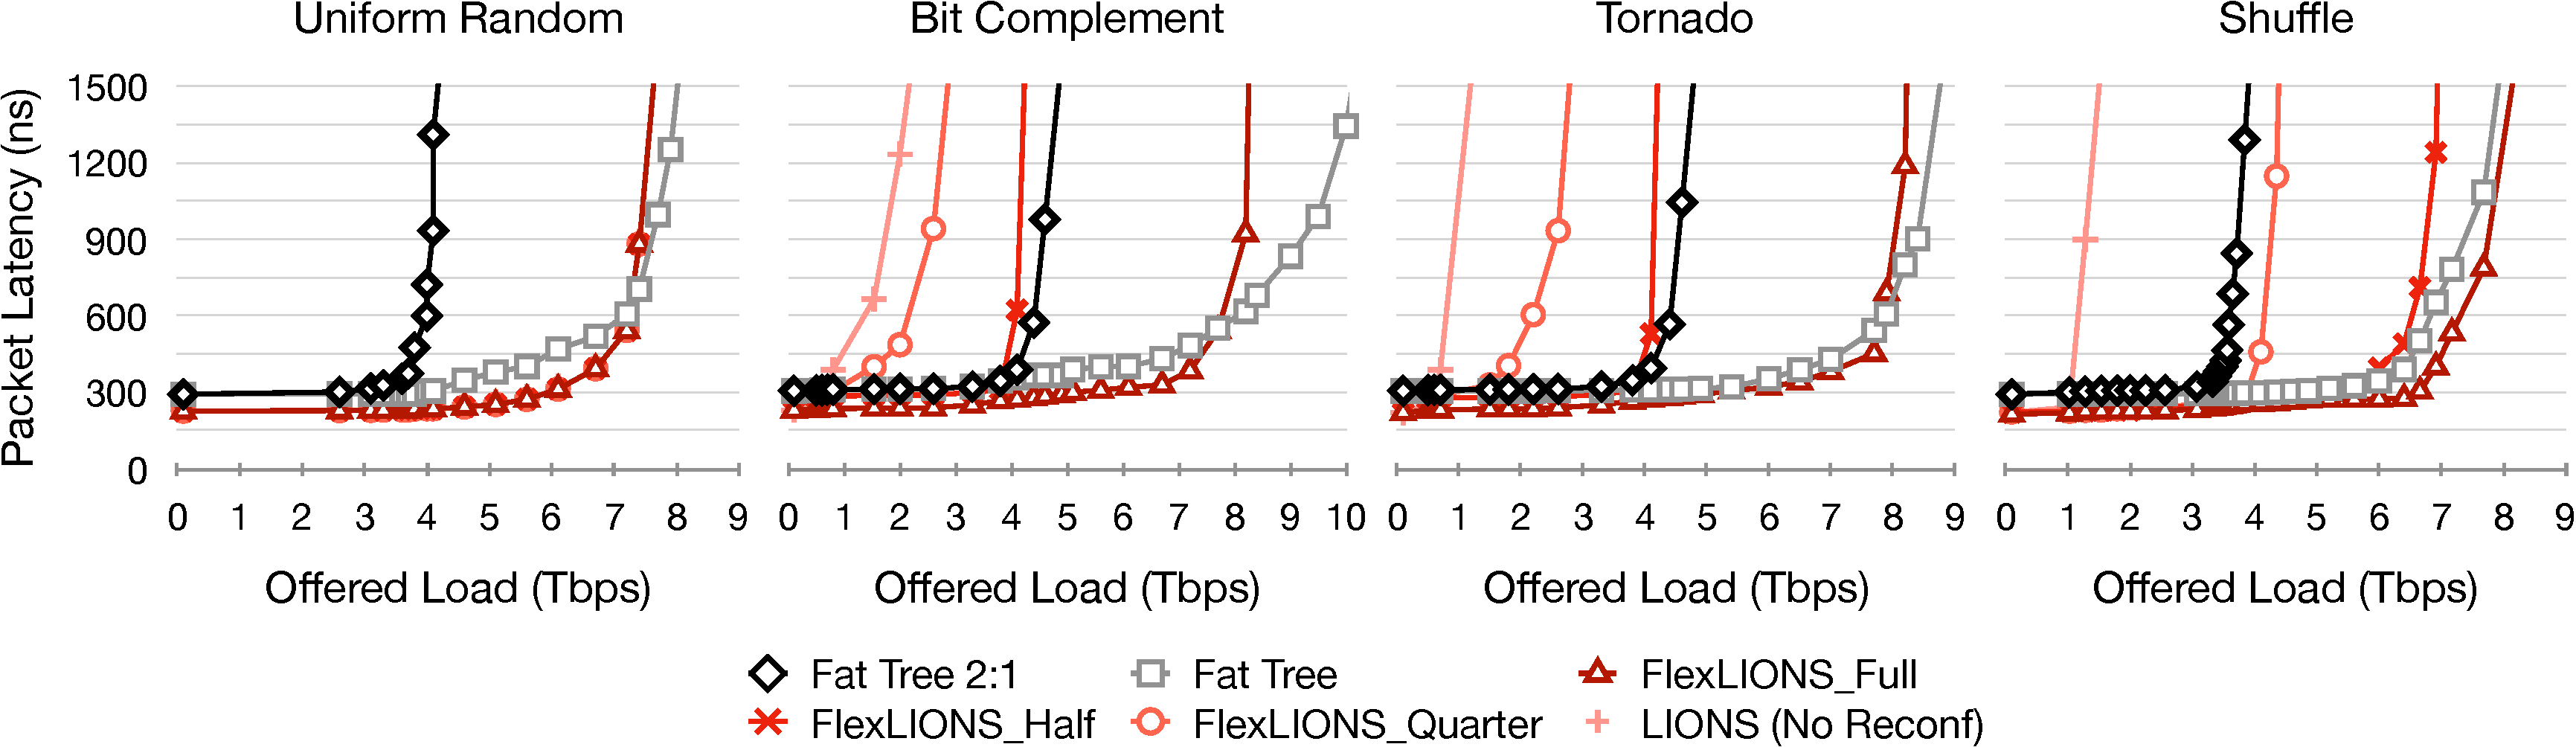
\includegraphics[width=\textwidth, clip]{Figures/syn.pdf}
        \caption{Average packet latency (ns) vs.\ offered load (Tbps) for different synthetic traffic patterns}
        		\label{fig:latsyn}
\end{figure*}
Given that the routing algorithms always choose the shortest path and that there is only one shortest path in an all-to-all network, LION without network configuration performs poorly for each traffic pattern aside from uniform random where traffic is evenly distributed across all links. Flexibility in bandwidth reconfiguration is therefore key if the traffic does not follow this corner case. For the different FlexLION reconfiguration capabilities, we observe that the more flexibility in the bandwidth assignment is available, the higher the total accepted traffic gets, which is in line with our hypothesis that fine-adjusting the bandwidth to links based on link utilization results in performance gains. \\
Compared to Fat Tree, which offers the same bisection bandwidth as FlexLIONS, FlexLION reduces the average packet latency prior to network saturation by 25\% on average which can be attributed to the lower average number of hops in FlexLION. FlexLION can compete with Fat Tree in terms of maximum throughput if it has full flexibility in terms of  wavelength reconfiguration for most traffic patterns. Compared to Fat Tree 2:1--a more light-weight implementation of the full Fat Tree--FlexLION nearly doubles the total bandwidth, and can compete even for lower levels of reconfiguration. 

\subsection{Power Results}
\subsubsection{Energy-per-bit}
Figure~\ref{fig:epb} illustrates the energy-per-bit (EPB) of the considered networks and transceiver technologies. Energy was calculated based on a FlexLION switch enabling full bandwidth reconfigurability (i.e. each wavelength can be assigned to any output port). LION indicates a full-mesh without bandwidth reconfiguration capabilities where the bandwidth is evenly distributed over all output ports. 
\begin{figure}[t!]
    \centering
        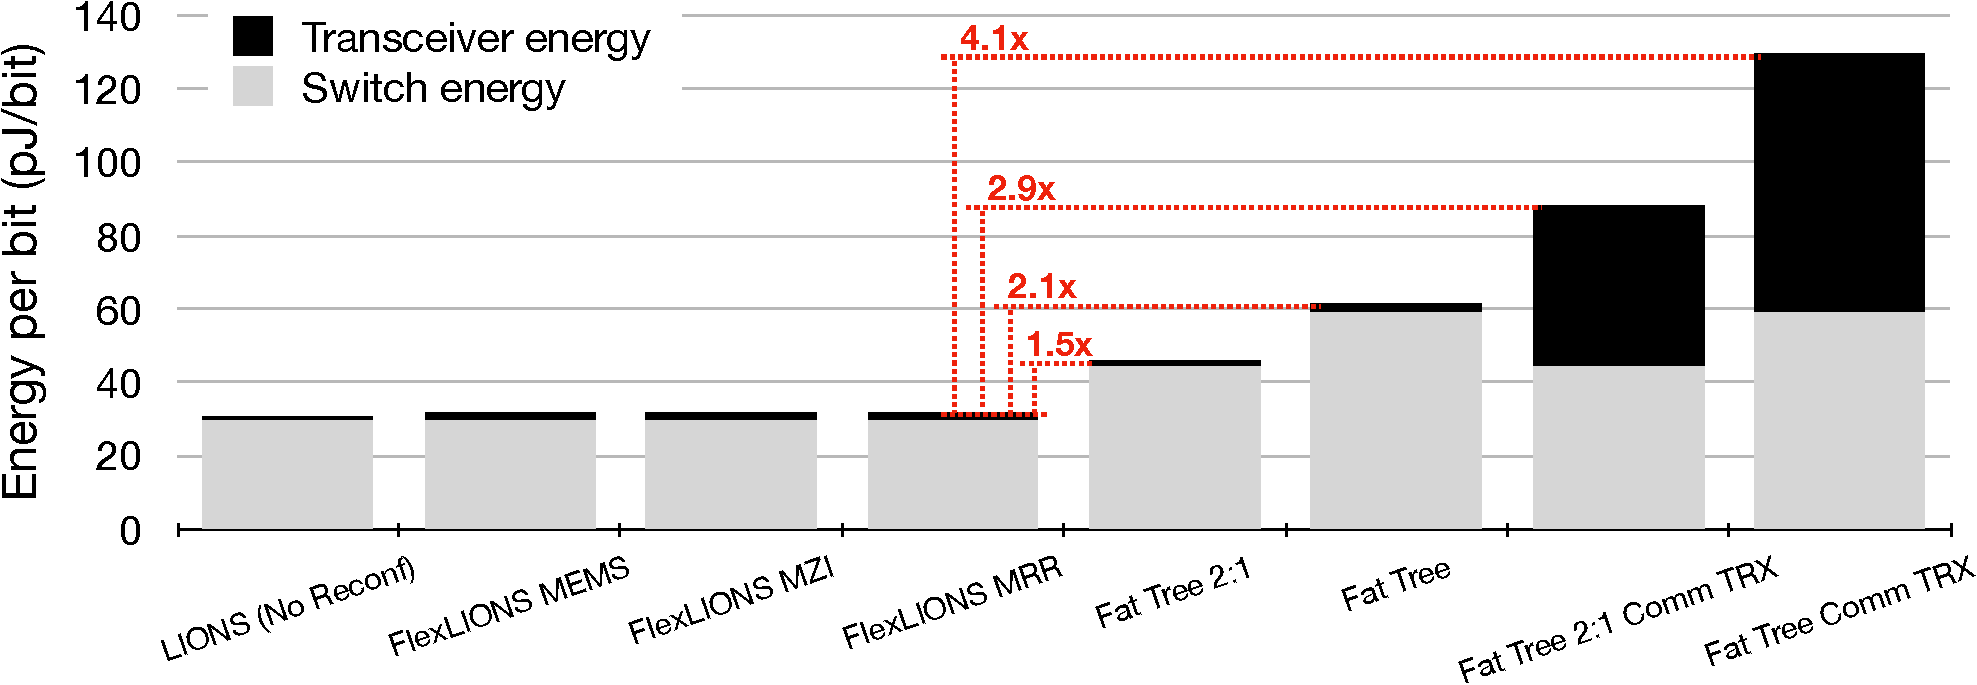
\includegraphics[width=\linewidth, clip]{Figures/epb.pdf}
    \caption[]{Energy-per-bit (pJ/bit) broken down into transceiver and switch energy of the different networks. `Comm' indicates commercially-available transceivers (TRX).}
    \label{fig:epb}
\end{figure}
The first observation is that the total energy is dominated by the network switches if the electronic-photonic co-designed transceivers are used. In this case, the reductions in power consumption between FlexLION and the fat tree topologies (2.1x (fat tree) and 1.5x (fat tree 2:1)) mostly comes from the energy saved by requiring fewer switches in the topology. \\
Depending on the color-blind switched used, FlexLIONS incurs higher losses and, in turn, higher power consumption. From a theoretical point of view, MEMS incurs the lowest loss of all color-blind switches (0.63dB vs. 2.16dB (MZI) and 2dB (MRR)); however, the high energy efficiency of the transceivers makes the energy differences of the different FlexLION designs negligible in the context of the whole network. The same applies to the degree of reconfiguration capability: the larger number of MRRs necessary to provide higher degree of flexibility cause higher path losses and higher power thermo-optical control of MRRs, but those impose negligible power overheads in a HPC network scenario, making FlexLIONS with full reconfigurability always the best design choice. \\
Compared to fat tree topologies with commercially-available transceivers, FlexLION offers up to 4.1x power reduction indicating the big impact that FlexLION could have compared to legacy designs. 

\subsubsection{Throughput-per-Watt}
Figure~\ref{fig:tpw} illustrates the TPW (maximum sustained throughput divided by power consumption) for the different network designs. Note that the power consumption for FlexLION's TPW values is based on a MEMS implementation (we omit the MZI and MRR based designs for simplicity as the difference in power consumption is $<$1\% and has a negligible impact on TPW). 
\begin{figure}[t!]
    \centering
        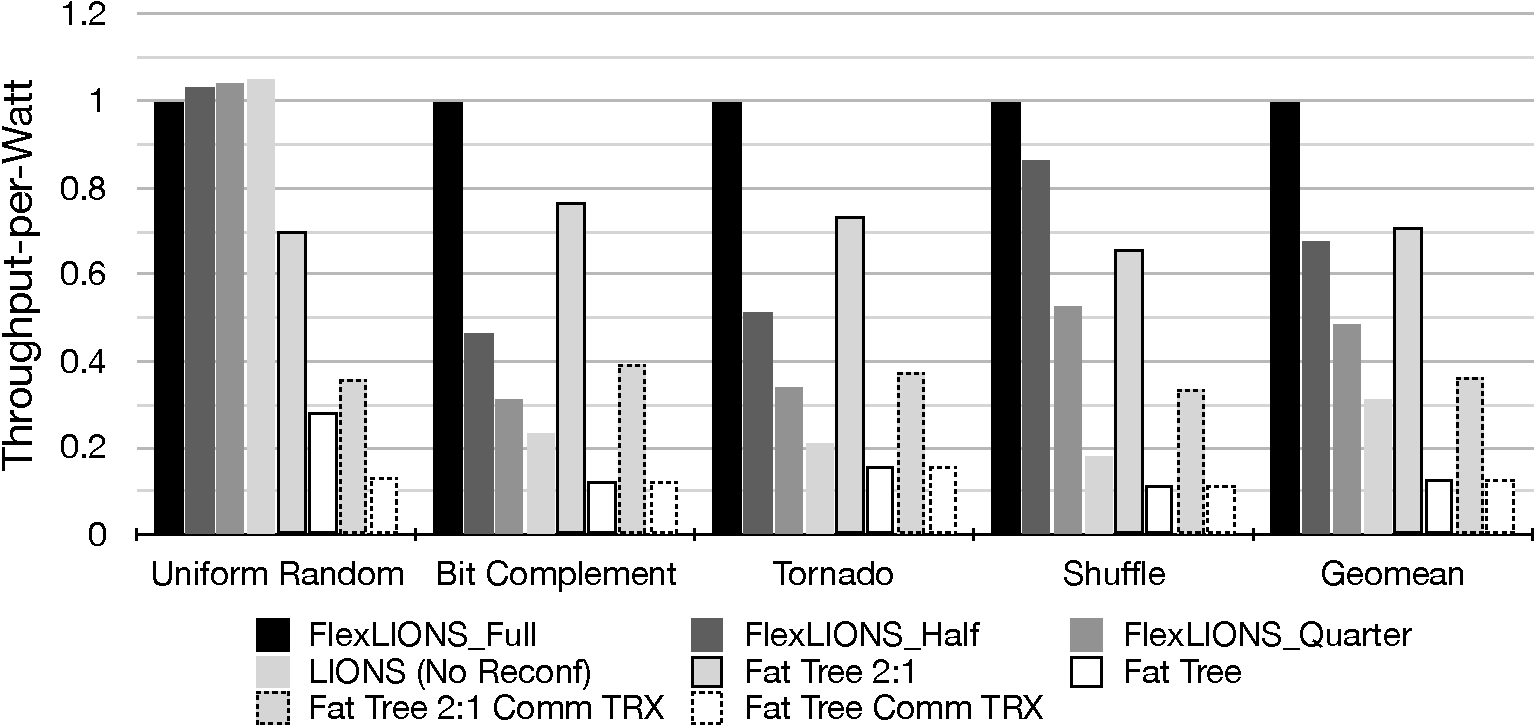
\includegraphics[width=\linewidth, clip]{Figures/tpw.pdf}
    \caption[Throughput-per-Watt (measured with maximum sustained throughput divided by power consumption) for the  different network designs normalized to FlexLION.]{Throughput-per-Watt (measured with maximum sustained throughput divided by power consumption) for the  different network designs normalized to FlexLIONS.}
    \label{fig:tpw}
\end{figure}
FlexLION outperforms all other designs significant on all traffic patterns. Fat tree 2:1 is the closest competitor but only exhibits 0.7x of FlexLIONS's TPW. Though supporting much less maximum throughput, Fat Tree 2:1 is actually more power efficient than a full Fat Tree as it saves a lot of power through exhibiting fewer switches and transceivers. In fact, our TPW results reveal that Fat Tree 2:1 would actually be more power efficient than FlexLIONS with reduced bandwidth reconfiguration capability, which waste much of their bandwidth on barely-utilized links. The network bandwidth reconfigurability of FlexLION is thus not only beneficial in terms of power efficiency, but also necessary to compete with state-of-the-art HPC networks. \\
In fact, unless traffic is perfectly uniformly distributed (in which case FlexLION without reconfigurability capability is the most power efficient as it provides the same throughput at reduced power), power efficiency in FlexLION is always the best with maximum flexibility in reconfiguration. However, such traffic patterns are very uncommon in HPC networks and are therefore of low practical relevance. 

\subsection{Discussion}
FlexLION interconnection fabric allows for all-to-all connectivity and full, fine-grained bandwidth reconfigurability from each input to each output port while successfully supporting line rates of 100Gb/s (as in legacy HPC interconnects). This fabric allows to significantly reduce the number of electronic switches and transceivers in HPC networks while providing similar maximum throughput at lower latency. While Fat Trees--the de-facto standard for HPC networks--offer a scalable fabric and load balancing, their resource requirements and higher network diameter make them inferior to FlexLIONS. \\
Effectively, FlexLION tightly-integrated and bandwidth-flexible fabric allows to reduce the stages in a multi-stage topology like trees and could therefore also be integrated as a part of a bigger HPC network. While our results confirm its efficiency for interconnecting 256 nodes, FlexLION could theoretically also scale to larger node counts; however, at some point the number of required wavelength in the network puts an upper limit on what is feasible and practical. At this point, a hierarchical topology approach will be needed--potentially with FlexLION at several levels of the hierarchy. \\
From a technology point of view, AWGR technology on silica and bulk optical MEMS technologies are currently commercially available; however, to reach the required level of integration with electronics discussed in this paper, SiN AWGR technology, integrated SiPh transceivers and SiPh color-blind switches are needed. Although successfully demonstrated, these technologies are still available only at the research level and practical issues as efficient thermal control, low crosstalk and low uniform loss require further research and engineering efforts from both academia and industry. However, our results suggest that once these technologies will transition from research to production level, they can have a significant impact on the energy efficiency, performance and scalability of future HPC systems thanks to their superior energy efficiency and bandwidth, low latency, and reconfigurability. 

\section{Related Work}
Several previous studies investigated the use of optics in HPC networks~\cite{perello2013all}, some in combination with electrical solutions~\cite{Farrington2010Helios}\cite{Wang2010cthrough} (referred to as \textit{hybrid}) while others solely rely on optical components~\cite{Mellette2017RotorNet}\cite{Chen2014OSA} as the interconnect. \\
Helios~\cite{Farrington2010Helios} is a hybrid approach based on a 2-layer tree that combines conventional electrical packet switches with optical circuit switches based on MEMS. Although supplementing a traditional tree network with optical MEMS switches was shown to reduce power consumption and the number of switching elements, the circuit-switched approach of MEMS switches does not provide the flexibility and thus the performance of FlexLIONS. \\
Researchers at UC San Diego also proposed the use of optical circuit switching with their design RotorNet~\cite{Mellette2017RotorNet} which iterates over a fixed, static set of pre-determined optical port matchings to provide uniform random bandwidth across all endpoints. These rotations are done in a traffic agnostic manner to eliminate the need for a centralized control plane. While this approach overcomes some of the main challenges of circuit-switched solutions (i.e., only point-to-point connectivity), it fails to address needs of latency-sensitive HPC workloads. \\ 
OSA~\cite{Chen2014OSA} is another architecture taking advantage of MEMS switches and also makes use of wavelength selective switches to achieve dynamic topology reconfiguration by exploiting spatial and wavelength switching. In OSA, P out of N available ports in MEMS can be connected to each node. Parameter P defines the upper limit in number of nodes one node can connect to, but also affects the total number of nodes connected to one MEMS switch. Therefore, OSA comes with a trade-off between the total number of nodes and the amount of connectivity one system can achieve.\\
Rather than studying opportunities of integrating SiP switches into HPC networks, several studies have been dedicated to the design and implementation of the SiP switches itself. The most popular approach found in literature is the use of broadband ring resonators~\cite{DasMahapatra2014BroadMR}\cite{nikolova2017modular} which can be reconfigured to either drop or let pass the whole spectrum of wavelengths in a network from one waveguide to another, allowing to reconfigure arbitrary interconnections inside a switch. One  drawback is, as discussed earlier, the fact that BRRs are colorblind and do not allow fine-grained switching (and thereby limit the flexibility of a fabric for bandwidth reconfiguration). Besides, the number of BRRs required in an all-to-all switch grows quadratically with the number of ports, severely limiting its scalability. The main disadvantage of relying of a large number of BRRs, however, is that thermo-optic control for large numbers of BRRs is extremely challenging and impractical. \\
Finally, AWGRs-based data center switches have also been proposed in the scientific literature~\cite{proietti2018experimental}~\cite{cao2015hi}\cite{cao2015experimental}\cite{yin2013lions}\cite{proietti2013scalable} and generally seem to be very efficient in providing all-to-all switching capability with low crosstalk and loss. However, as described earlier, AWGRs alone can only provide the interconnection of nodes and, as a passive platform, cannot be reconfigured to adapt to varying communication demands. Nevertheless, FlexLIONS showed that the combination of AWGRs, MEMS, and MRs results in a powerful switch fabric exploiting the benefits of each SiP device. 

\section{Conclusion}
This paper presented FlexLION, a silicon-photonic interconnect fabric enabling all-to-all connectivity and bandwidth steering. FlexLION exploits the co-integration of AWGRs, MRs and spatial switches on the same chip to construct a flexible and energy-efficient interconnection fabric. When implemented as part of an HPC network, we found that FlexLION can reduce latency by 25\% and energy-per-bit  by up to 6.2x while sustaining similar maximum throughput compared to state-of-the-art tree-based topologies. Energy savings mainly come from the higher link utilization FlexLION offers, which in turn enables a network with fewer switches and transceivers. FlexLION fits on a $12mm \times 13mm$ interposer and can be reconfigured within just 1$\mu$s. Therefore, it is not only restricted to HPC networks, but may also be suitable for networks lower down the hierarchy, e.g. for on-board connectivity between multiple processors and memories or for intra-rack communication. 

\IEEEpeerreviewmaketitle

\bibliographystyle{IEEEtran}
\bibliography{references}

\end{document}


